\documentclass[conference]{IEEEtran}
\IEEEoverridecommandlockouts
% The preceding line is only needed to identify funding in the first footnote. If that is unneeded, please comment it out.
\usepackage{cite}
\usepackage{amsmath,amssymb,amsfonts}
\usepackage{algorithmic}
\usepackage{graphicx}
\usepackage{textcomp}
\usepackage{xcolor}
\usepackage{hyperref}
\usepackage{multirow}
\usepackage{fancyhdr}
\newcommand{\linebreakand}{%
  \end{@IEEEauthorhalign}
  \hfill\mbox{}\par
  \mbox{}\hfill\begin{@IEEEauthorhalign}
}

\def\BibTeX{{\rm B\kern-.05em{\sc i\kern-.025em b}\kern-.08em
    T\kern-.1667em\lower.7ex\hbox{E}\kern-.125emX}}
\pagestyle{fancy}
\fancyhf{}
\rfoot{Mentor: Prof. Jayprakash Lalchandani\\
Email: jayprakash\_lalchandani@daiict.ac.in}
\begin{document}
\title{SAH-YOJANA \\
\large {Helps you make the right choice}
}


\author{\IEEEauthorblockN{1\textsuperscript{st} Aniket Kaduskar}
\IEEEauthorblockA{201701005@daiict.ac.in}
\and
\IEEEauthorblockN{2\textsuperscript{nd} Yashvi Shah}
\IEEEauthorblockA{201701045@daiict.ac.in}
%\linebreakand
%\IEEEauthorblockN{Mentor: Prof. Jayprakash Lalchandani}
%\IEEEauthorblockA{jayprakash\_lalchandani@daiict.ac.in}
}

\maketitle
\begin{abstract}
This document is regarding the whole work done to
build a website which will recommend the government schemes to its user based on their profile. The document discusses the motivation, implementation, features and the importance of website.\\
\end{abstract}
\begin{IEEEkeywords}
Yojana Recommendation Portal, Javascript, Firebase
\end{IEEEkeywords}

\section{INTRODUCTION}
Government has launched a lot of schemes as a welfare measure, for its citizen, to provide social security and improve the quality of life for its people. But most of the time these benefits do not reach its beneficiary because the process is quite tedious. The citizens have to go through website of each and every scheme time and again and check for the eligibility and guidelines.\\ SAH-YOJANA can be of great help in such a case. The main aim of building this website as described by its tag line "Helps you make the right choice", was to provide citizen with a single destination to look for all the schemes launched by the government and ease up the process of searching through various schemes which he/she can apply by providing recommendations. The user just has to enter a few basic details and then the schemes will be recommended to the user based on the profile. The user can then directly apply for the scheme on the official government website. The portal helps to shorten the procedure and saves a lot of time for the user. 
\begin{figure}[h!]
\centering
\fbox{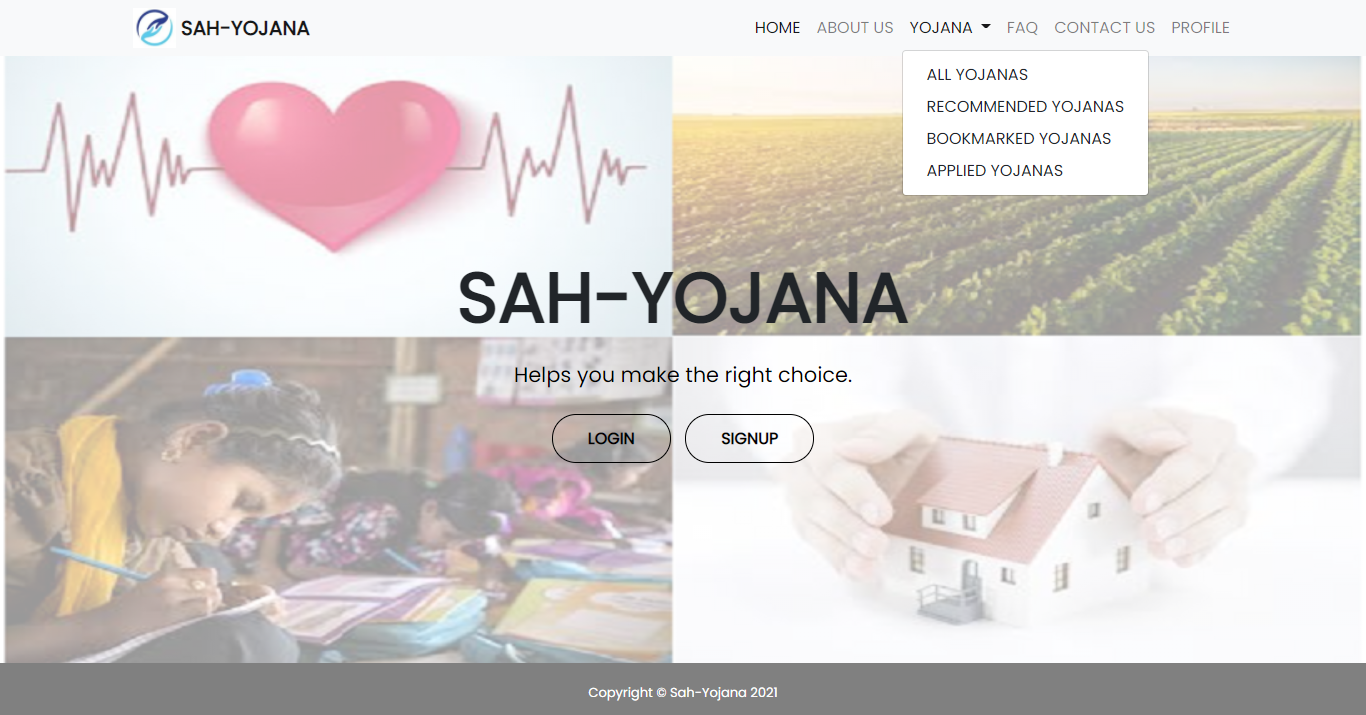
\includegraphics[width=0.45\textwidth]{home_screen (2).png}}
\caption{Home Screen of SAH-YOJANA}
\end{figure}
After the application the user can also keep track of the list of schemes he/she has applied and can also check the application status through the portal itself. Thus SAH-YOJANA can help the citizens to take utmost benefits of schemes and it served as the main motivation for us to build the website. 


\section{OUR APPROACH}
The first step was to gather all the requirements for the website at the basic level by listing down the user stories. In order to get a clearer picture of the website, UI design of the website was created along with different UML diagrams like activity diagram, use case diagram, sequence diagram etc which are shown in Appendix below. Then after, we researched for the different tools and technology available and the best that could be used by us to develop the website based on our requirements. After that, the development phase started and we started developing the sections of the website according to the functionalities decided beforehand. Once the website was developed, we tested it and based on the feedback the necessary improvements were done and the website was finally ready to be deployed.

\section{USER STORIES}
\begin{itemize}
    \item As an unregistered user, I can sign up on the portal.
    \item As a user, I can login on the portal so that I can take the utmost benefit of the government schemes.
    \item As a user, I can logout from the portal.
    \item As a registered user, I can edit my profile in order to receive recommendations about the eligible schemes.
    \item As a user, I can search schemes using the search bar.
    \item As a user, I can filter the schemes based on domains.
    \item As a registered user, I can bookmark the schemes so that I can revisit them later and apply for them.
    \item As a user, I can look for answers to frequently asked questions.
    \item As a user, I can look up for the detailed information of every scheme including description, eligibility criteria, guidelines,video etc. on the scheme page and apply for the scheme.
    \item As a registered user I will get recommendations for schemes based on my profile.
    \item As a registered user, I can receive emails when a new yojana is announced.
    \item As a user, I can get the locations of government offices where I can get help for these yojanas.
    \item As a user, I can add a complaint on the portal and receive a reply through email notification.
    \item As a registered user, I am prompted when I login to the portal whether I applied to any particular yojana or not, if I have visited the official govt. website through the portal.
    \item As a registered user, if I enter 'yes' in the prompt, then a feedback form regarding the application process, problems faced and the benefits received is emailed to me.
    \item As a registered user, I can keep track of all the yojanas to which I have applied also check for the application status if online tracking is available.
    \item As an admin, I can add yojanas to the portal.
    \item As an admin, I can remove yojanas from the portal.
     \item As an admin, I can enable a yojana
    \item As an admin, I can disable a yojana.
    \item As an admin, I can update the details of yojana along with the eligibility criteria.
    \item As an admin, I can view the complaints submitted by the users and reply them back with the correct guidelines.
    \item As an admin, I can view the total users, active users, active yojanas, inactive yojanas, domain wise count of yojanas, total complaints lodged, complaints resolved on the portal.
    \item As an admin, I can download a report of the count of users who have bookmarked/applied to a particular scheme.
    \item As an admin, I can see the feedback responses of the users from the portal itself.
    

\end{itemize}
\section{FUNCTIONAL DESCRIPTION THROUGH THE USE CASES}
In this section, the main functionalities provided by the website are explained. Along with this other basic functionalities like FAQ page, Contact Us page, About Us page are also included in the website. The website has two stakeholders, the user and the admin. First the functionalities provided to the user are discussed:\\
\subsection{USER}
\subsubsection{Signup / Login}
In order to get recommendations the user needs to first register on the portal. For registration, the user will have to provide his name, valid email address and password. After registration, the user will be sent an authentication mail on his/her registered email ID and after clicking the verification link the user will be able to login into the portal to use various functionalities. 
\begin{figure}[h!]
\centering
\fbox{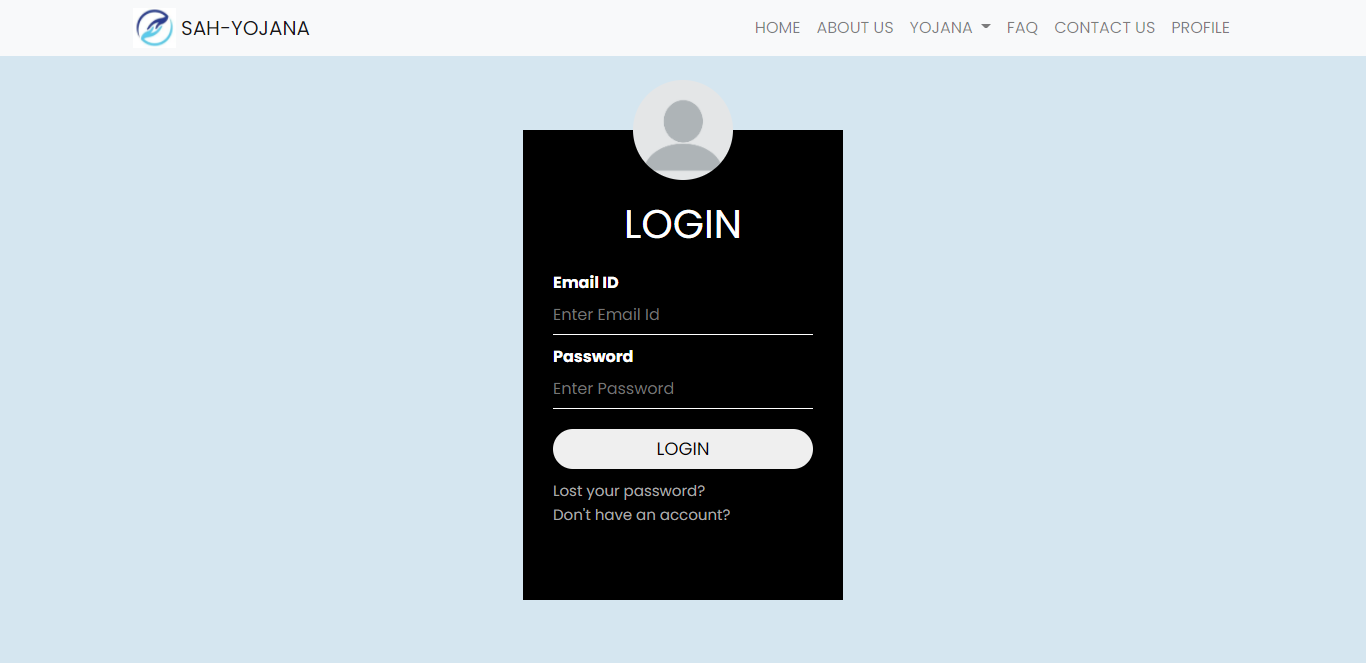
\includegraphics[width=0.45\textwidth]{login.png}}
\caption{Login Page}
\end{figure}
Validation feature is also implemented in the sign up page in order to make sure that the details entered are in the correct format for fields like email ID and password. The user can also log out from the current session and prevent access by any other user without valid credentials.
\begin{figure}[h!]
\centering
\fbox{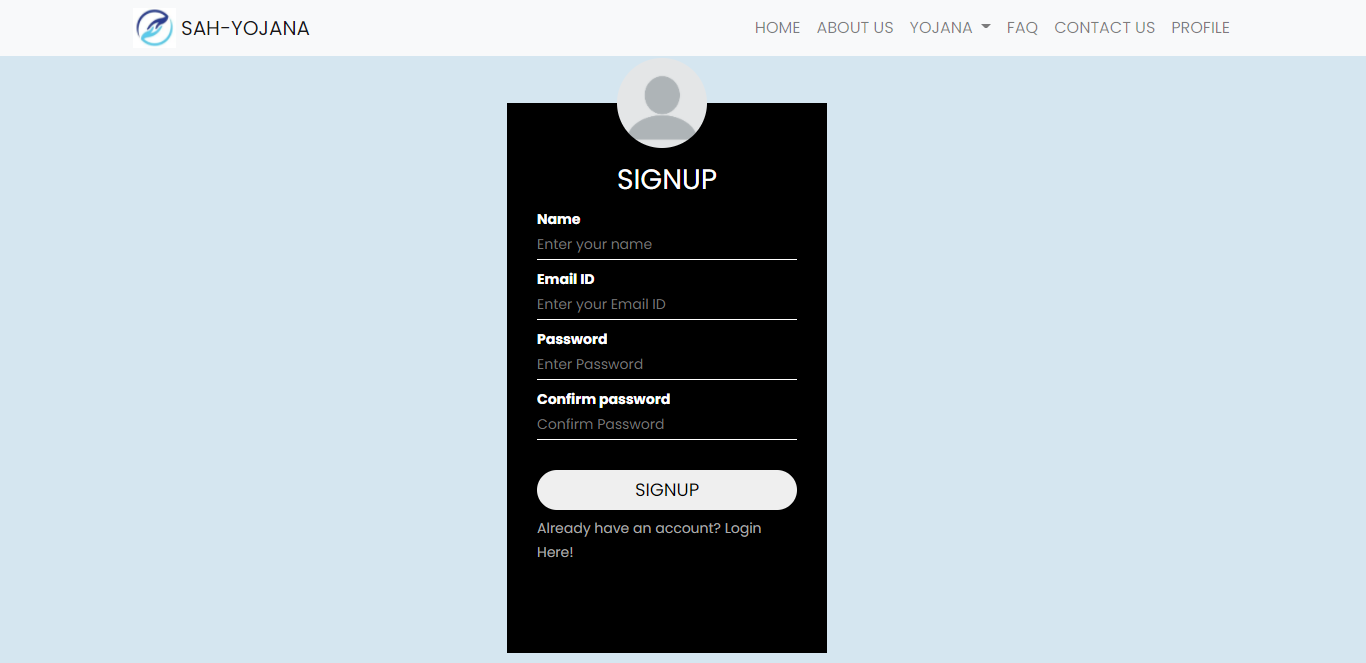
\includegraphics[width=0.45\textwidth]{signup (2).png}}
\caption{Signup Page}
\end{figure}
\subsubsection{Forgot Password}
In case the user has registered but forgot the password used for login, he/she can visit the forgot password page where he/she will receive a reset password link through email after entering the registered email ID. Thus the password will be changed and thereafter the user can log in using the new password.

\begin{figure}[h!]
\centering
\fbox{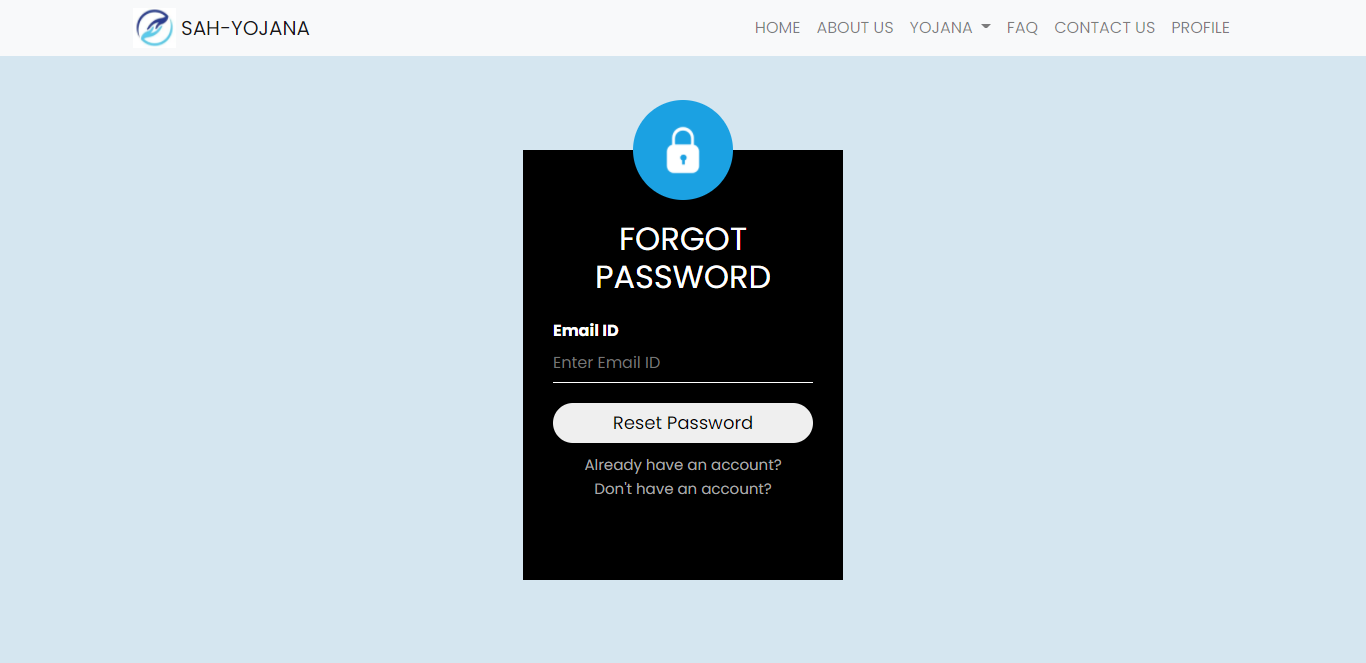
\includegraphics[width=0.45\textwidth]{forgot_password.png}}
\caption{Forgot Password Page}
\end{figure}
\subsubsection{Profile}
\paragraph{Create Profile}
If the user has logged in for the first time he/she will be redirected to create profile page, where the user will have to enter his personal information like age, gender, details regarding his/her occupation based on which the user will receive the recommendations. Alert will be shown if any of the fields are empty. 
Recommendations will only be received on completing the profile. If the user has not done so he/she will always be prompted to complete the profile after log in as well as when he/she wishes to visit the "Recommended Yojanas" page.
\begin{figure}[h!]
\centering
\fbox{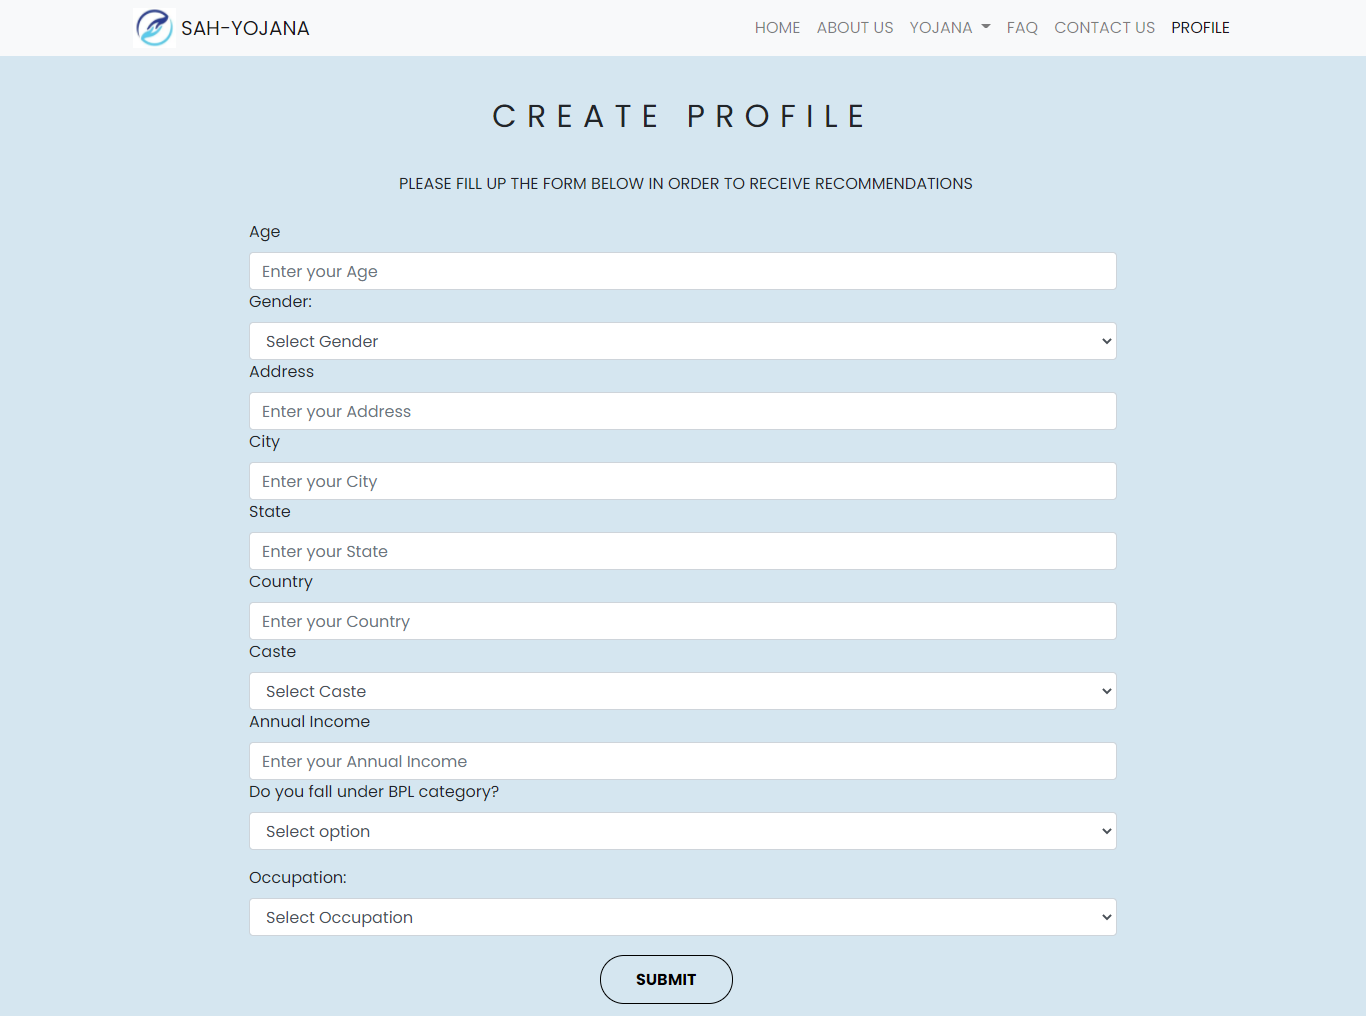
\includegraphics[width=0.45\textwidth]{create_profile.png}}
\caption{Create Profile Page}
\end{figure}
The create profile page is designed dynamically as it adapts according to the answers entered by users, for example if the user enters it's occupation as a student the form will change and ask for the details pertaining to a student like standard, school etc.
\paragraph{Edit Profile}
Once the user has completed the profile, he/she is also given the option of editing a few fields which are subject to change like age, occupation, address etc. To edit the profile the user can visit the "Profile" tab  and save changes accordingly. The recommendations will be changed according to the new details entered by the user. 
\begin{figure}[h!]
\centering
\fbox{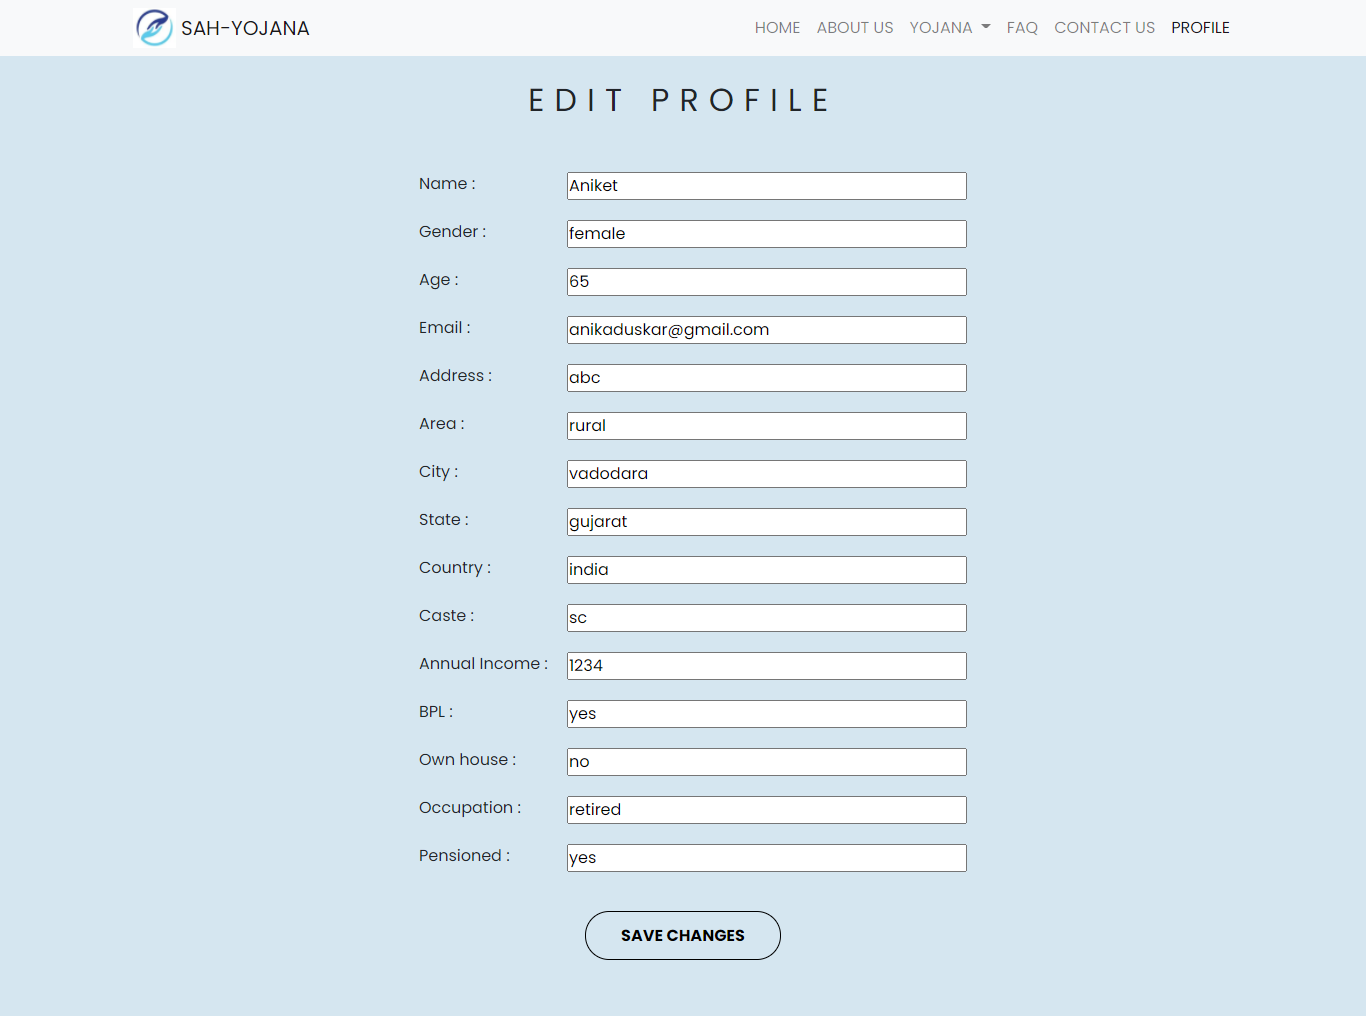
\includegraphics[width=0.45\textwidth]{edit_profile.png}}
\caption{Edit Profile Page}
\end{figure}
\subsubsection{Yojanas}
\paragraph{All Yojanas}
All Yojanas tab in the dropdown menu of Yojana tab in the navigation bar shows all the active schemes which are currently included on the portal. The schemes can be filtered based on the domains like agriculture, education, health etc. which can be done by choosing the filter which the user wants from the 'Categories' tab on the page.
\begin{figure}[h!]
\centering
\fbox{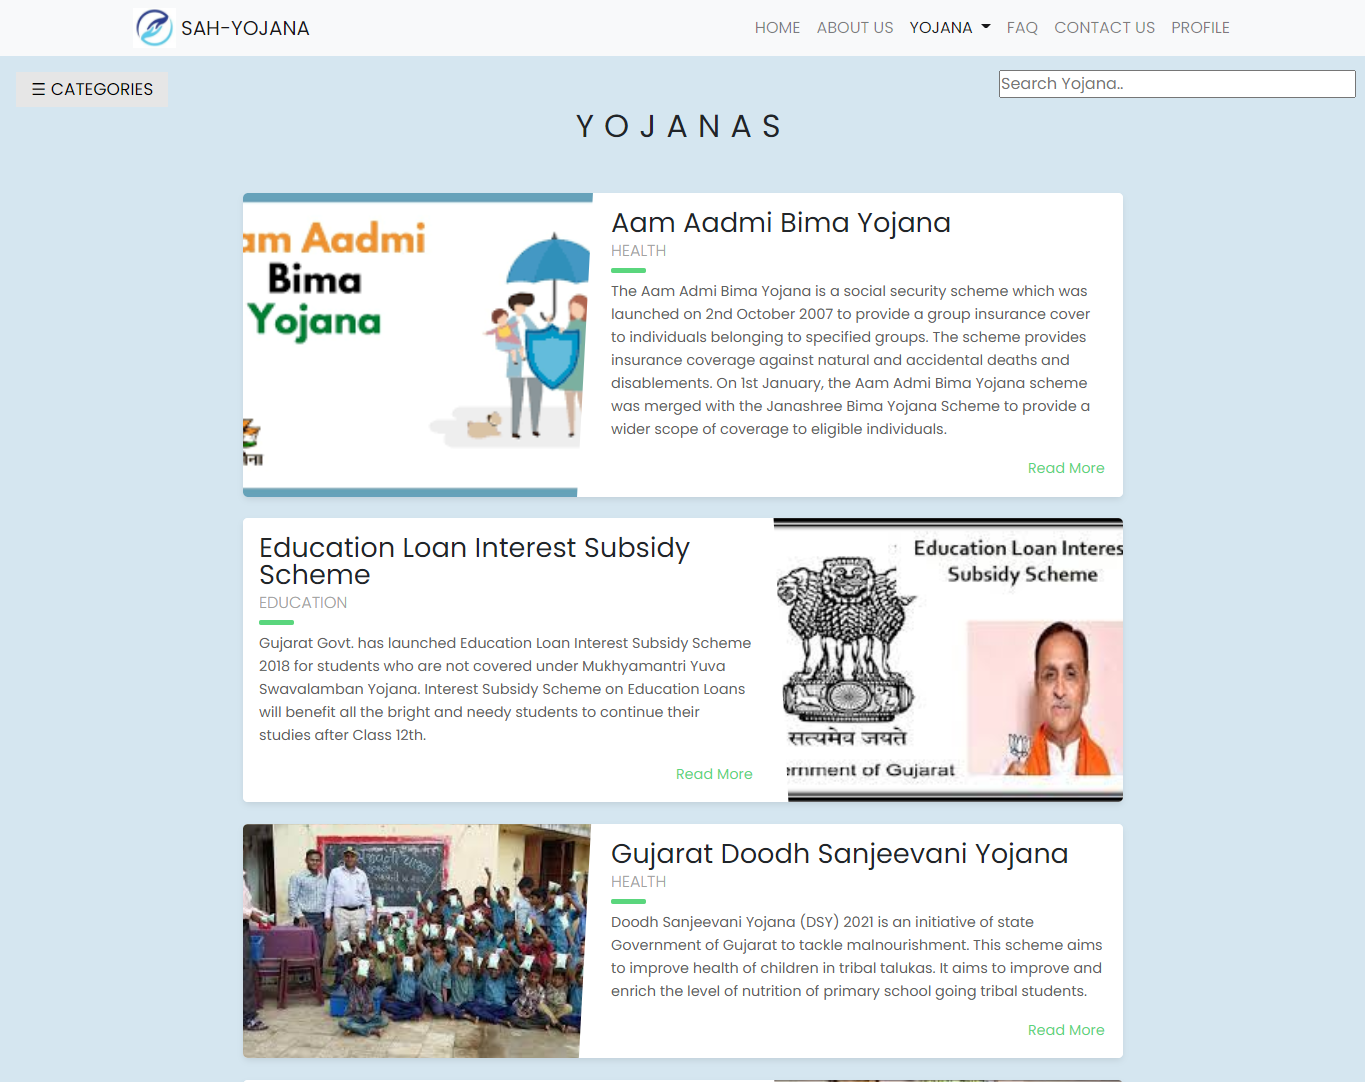
\includegraphics[width=0.45\textwidth]{Yojana.png}}
\caption{All Yojana Page}
\end{figure}
The user can search for a scheme using the search bar as well. Each scheme is displayed on a scheme card where a short information about the scheme is displayed along with a video link which can be accessed by hovering on the logo of scheme in that card. In order to view the detailed information the user can click read more link where the user will be redirected to a page which displays all the details of the scheme. 
\paragraph{Bookmarked Yojanas}
The portal also allows the user to bookmark a scheme and refer it later. If the scheme is already bookmarked the user will be shown an alert. 
\begin{figure}[h!]
\centering
\fbox{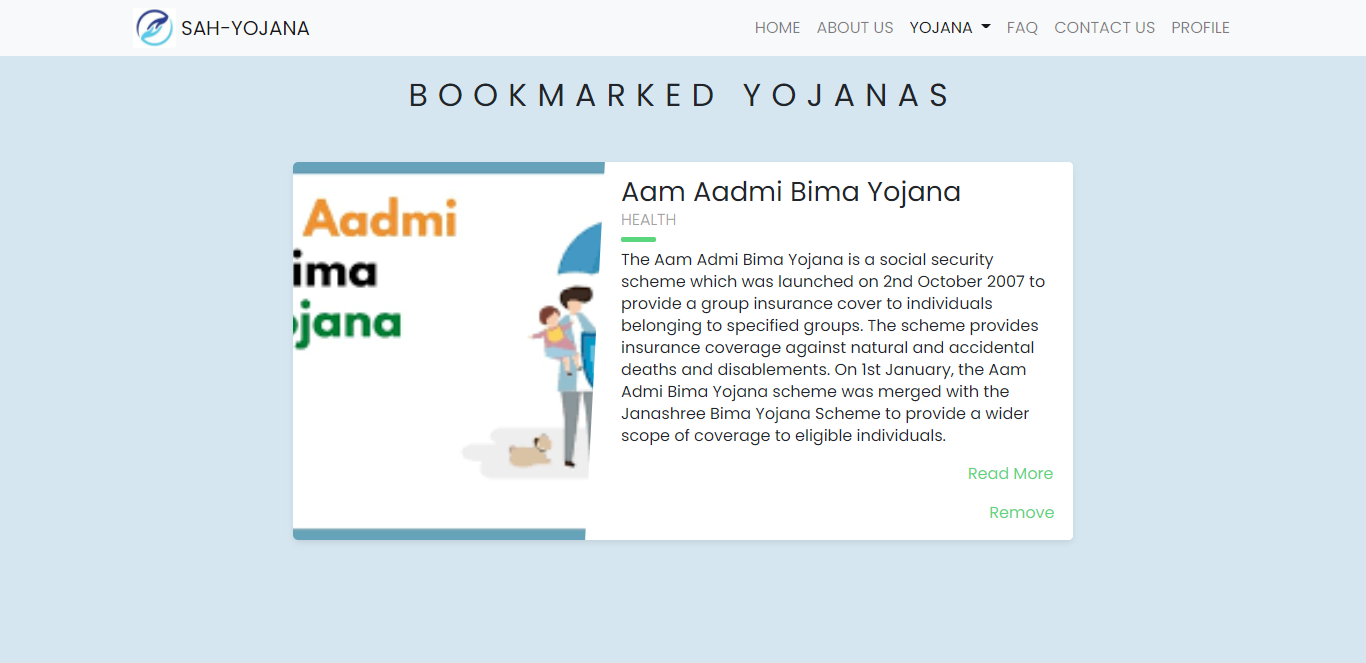
\includegraphics[width=0.45\textwidth]{bookmark.png}}
\caption{Bookmarked Yojanas Page}
\end{figure}
The user can see all bookmarked schemes by visiting 'Bookmarked Yojanas' tab in the 'Yojana' dropdown from the navigation bar. The user is also allowed to remove the scheme from bookmark as per the need.  
\paragraph{Recommended Yojanas}
When the user visits the "Recommended Yojanas" page, the user is displayed a list of all recommended schemes which are curated based on the details entered by the user in his profile. The user can then check for the details of the scheme, bookmark or apply for the scheme accordingly.

\begin{figure}[h!]
\centering
\fbox{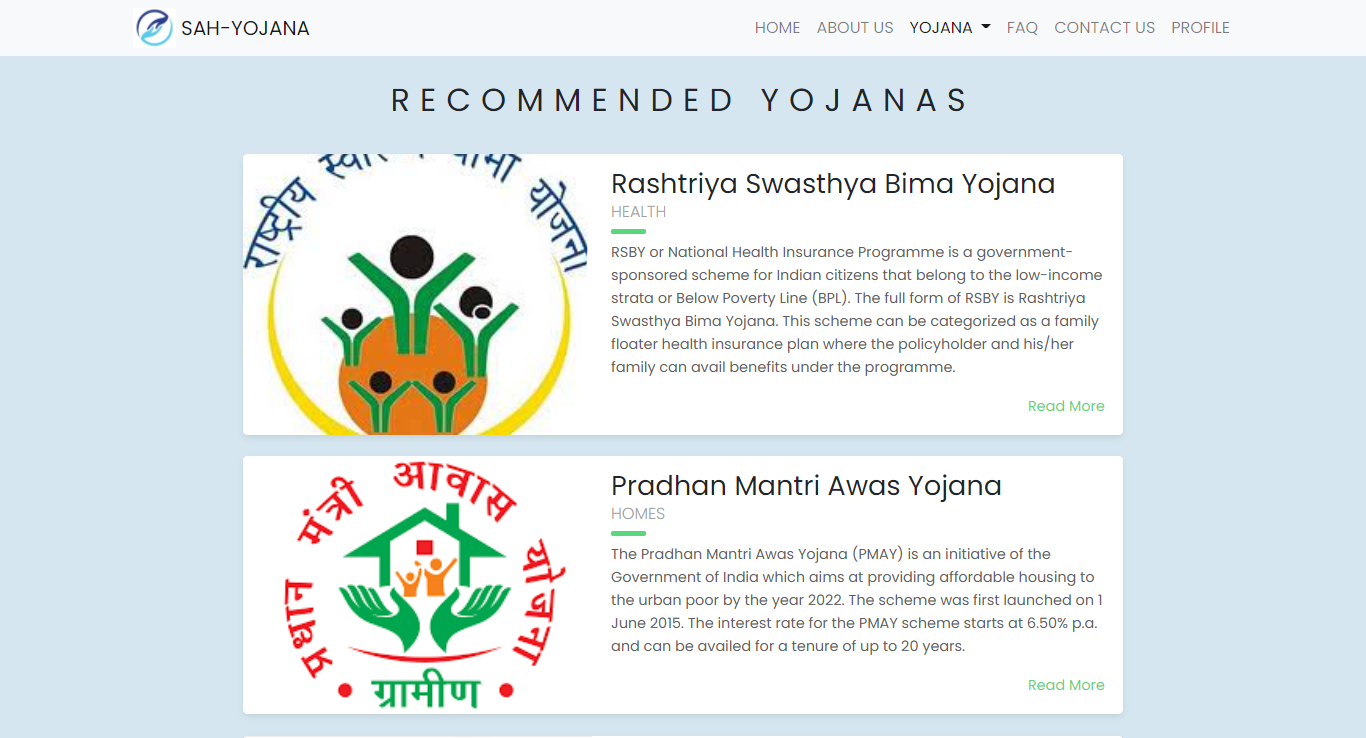
\includegraphics[width=0.45\textwidth]{reommend.png}}
\caption{Recommend Yojanas Page}
\end{figure}
\paragraph{Applied Yojanas}
This page keeps track of all the schemes applied by the user till now. The user can visit the page and click on the "Check application status" button to track the current status of the scheme. In case online tracking is not available for that particular scheme the user can also use the helpline number displayed on the scheme card to know the current status and get updates. The scheme card also displays application ID so that the user can refer it easily while checking for the status of application.

\begin{figure}[h!]
\centering
\fbox{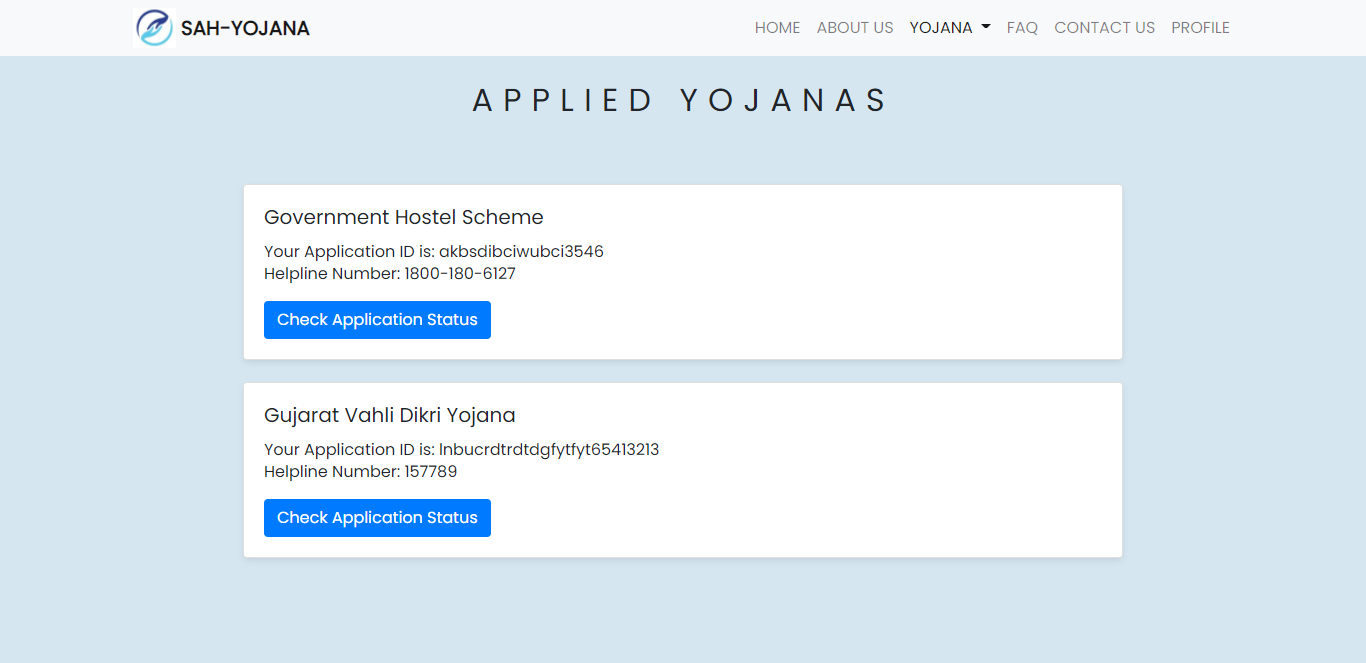
\includegraphics[width=0.45\textwidth]{applied_yojanas.png}}
\caption{Applied Yojanas Page}
\end{figure}

\subsubsection{Readmore Page}
After clicking on the 'Read More' link on the scheme card, the user will be redirected to a page which features detailed information regarding the scheme like description, guidelines, eligibility, along with an in frame video for easy understanding about the scheme. The user can bookmark schemes using the bookmark button. When clicked on the apply button the user will be redirected to the official government website for direct application.
\begin{figure}[h!]
\centering
\fbox{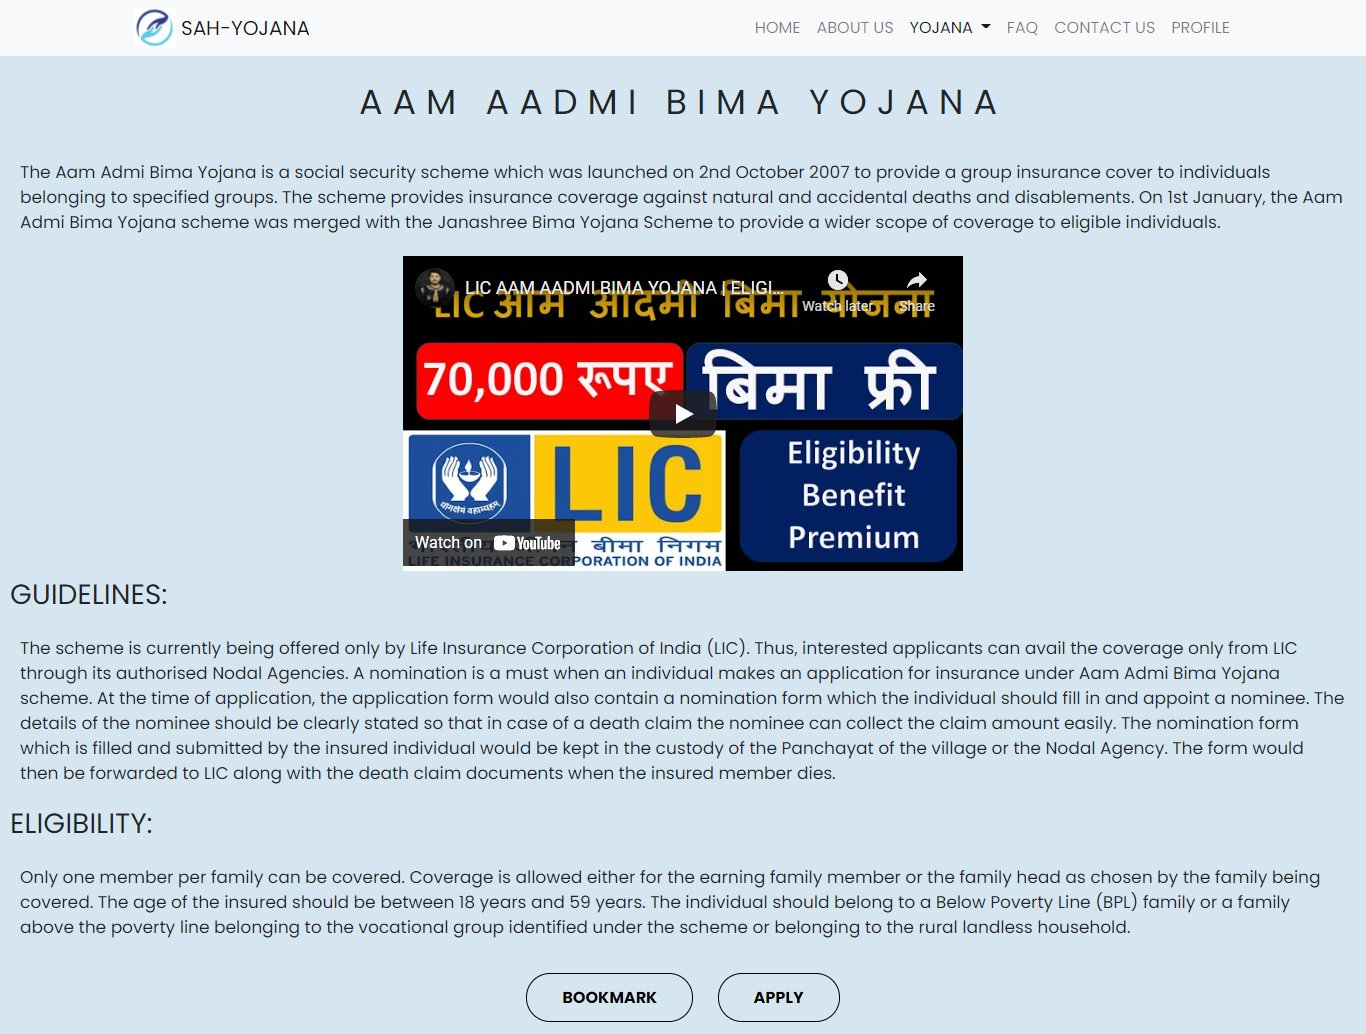
\includegraphics[width=0.45\textwidth]{read_more.png}}
\caption{Read More Page}
\end{figure}
\subsubsection{Tracking the application status}
The activity of the user visiting the official government application website through the portal is tracked and when the user logs in again to the portal he is prompted asking whether he has applied to the scheme or not. If the user enters 'Yes' then the scheme will be added to the 'Applied Yojanas' page of the portal. They will also be asked to enter the application ID so that they can easily use it for future reference while checking their application status. If the user enters 'Later' then the user will be prompted again the next time he logs in. If 'No' is entered, he will not be prompted again regarding the application unless he visits the official government website again through the portal.
\begin{figure}[h!]
\centering
\fbox{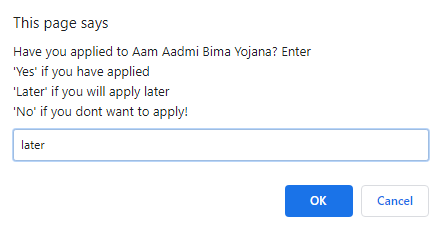
\includegraphics[width=0.45\textwidth]{prompt.png}}
\caption{Prompt to know if the user has applied or not}
\end{figure}
\paragraph{Feedback Form}
If the user has applied for a scheme, a feedback form regarding the application details, problems faced and the benefits received is emailed to the user.

\subsubsection{Contact Us Page}
The "Contact Us" tab on the navigation bar lists the address and email ID of the administration handling the website. 
\paragraph{Add complain}
The user can add a complaint regarding any issues related to the portal, application, guidelines or eligibility criteria of any scheme. For adding a complain, the user has to click on the 'Add a Complain' button on the Contact Us page where he will be redirected to a new page where he/she can enter the details of the issue and submit. The complaint will be then resolved by the admin and the user will receive a reply email from the admin regarding the complaint. Validation is implemented on the page to ensure that the details are filled in the correct format. Also a few fields are kept compulsory like email ID without which the complain will not be submitted.
\begin{figure}[h!]
\centering
\fbox{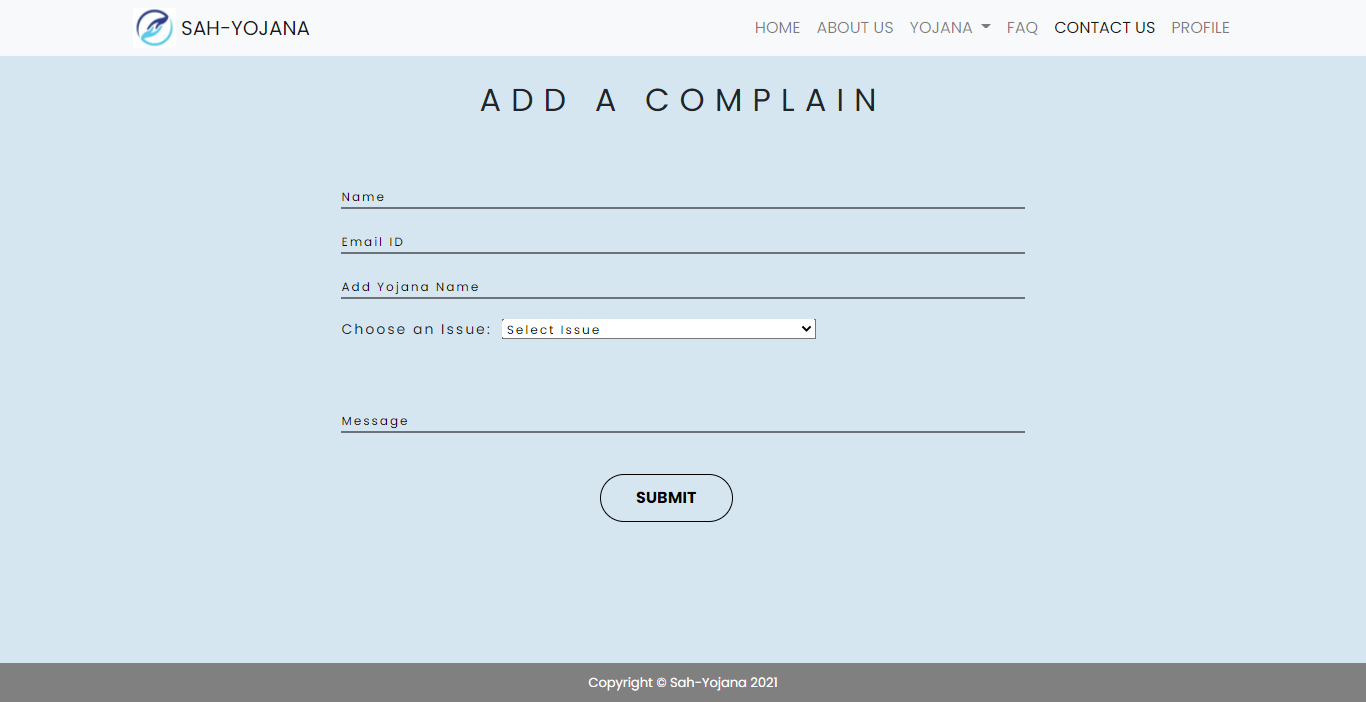
\includegraphics[width=0.45\textwidth]{complain.png}}
\caption{Add a Complaint Page}
\end{figure}
\paragraph{Map View}
If the user wants to get more information regarding the scheme or wants to apply for the scheme in person then the user can visit the government office in its nearby location. For this the portal helps the user by providing in frame map view of the location of government offices.
To access the map, user has to visit the "Contact Us" page and click on "Map View" to know the locations of government offices. The user can also know the exact location of the government office by clicking on the map marker which will display the address of the government office and the scheme which the office is accountable for.
\begin{figure}[h!]
\centering
\fbox{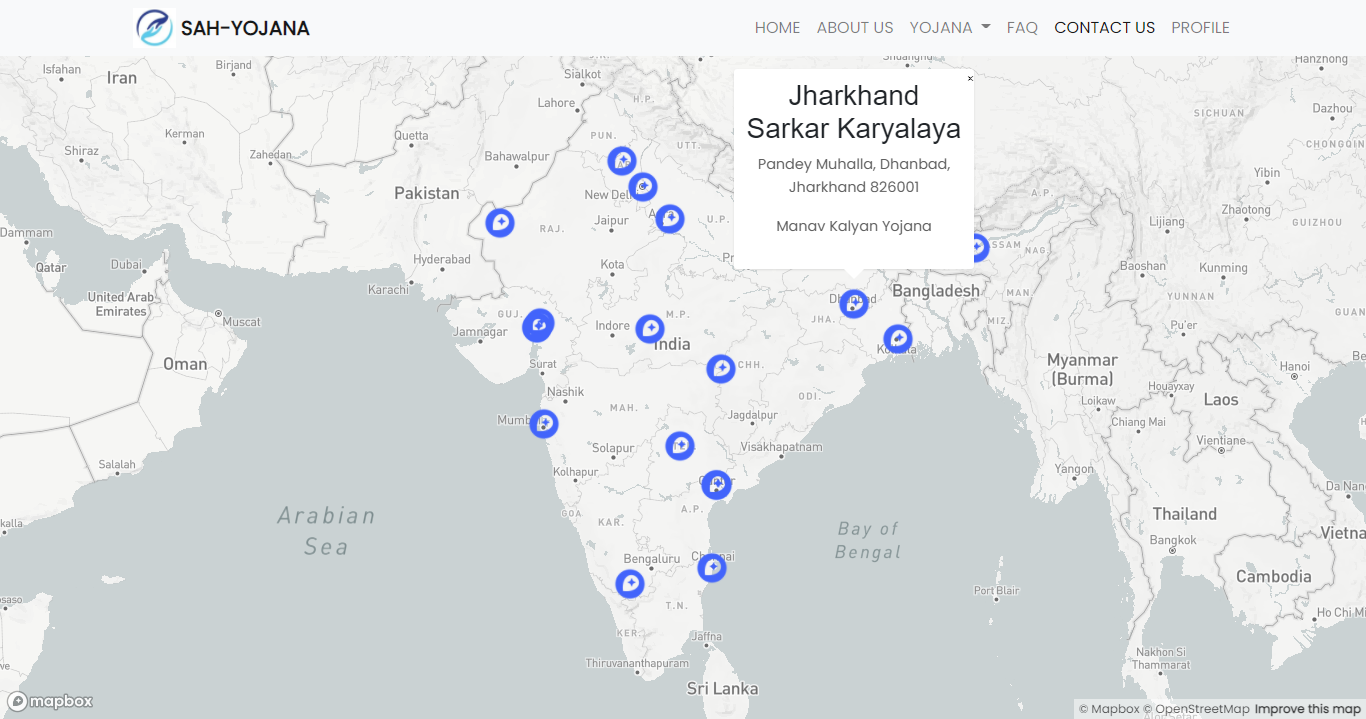
\includegraphics[width=0.45\textwidth]{map.png}}
\caption{Map View of Government Offices}
\end{figure}


\subsection{ADMIN}
\subsubsection{Login}
The admin need not sign up in the portal instead he/she is given the credentials before hand which can be used to login into the portal and access the functionalities of admin.
\subsubsection{Yojanas}
All the active schemes currently included on the portal are displayed on this page. The admin can search for any particular scheme using the search bar. The admin is given two options to add a new scheme to the portal. The admin can click on "Add Yojana" button and either enter a new scheme or enable an already existing scheme by clicking on "Add Existing Yojana" button. 
\begin{figure}[h!]
\centering
\fbox{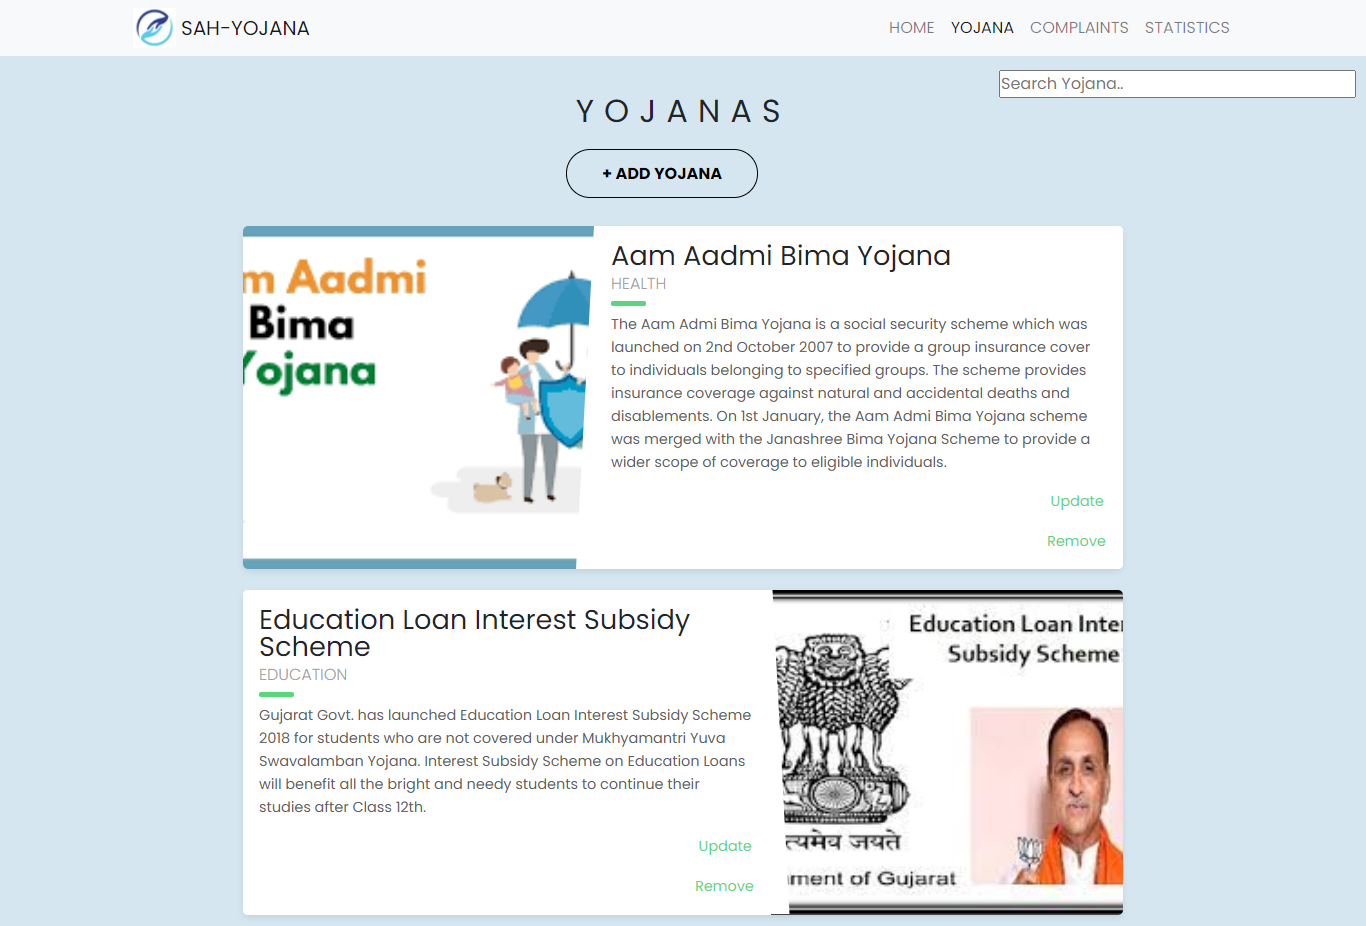
\includegraphics[width=0.45\textwidth]{admin_yojana.png}}
\caption{Yojana page of Admin}
\end{figure}
\paragraph{Add Yojana}
For adding a new scheme to the portal admin has to add all the details of the scheme like name, domain, description, guidelines, eligibility, image, video, application link etc. The admin also has to enter a semi-colon separated string of the eligibility criteria which will be matched with the profile of the user in order to recommend the scheme to a particular user. When a new scheme is added into the portal by admin the system will automatically send email notifications to all of its registered users about the addition of new scheme in order to keep them updated.
\begin{figure}[h!]
\centering
\fbox{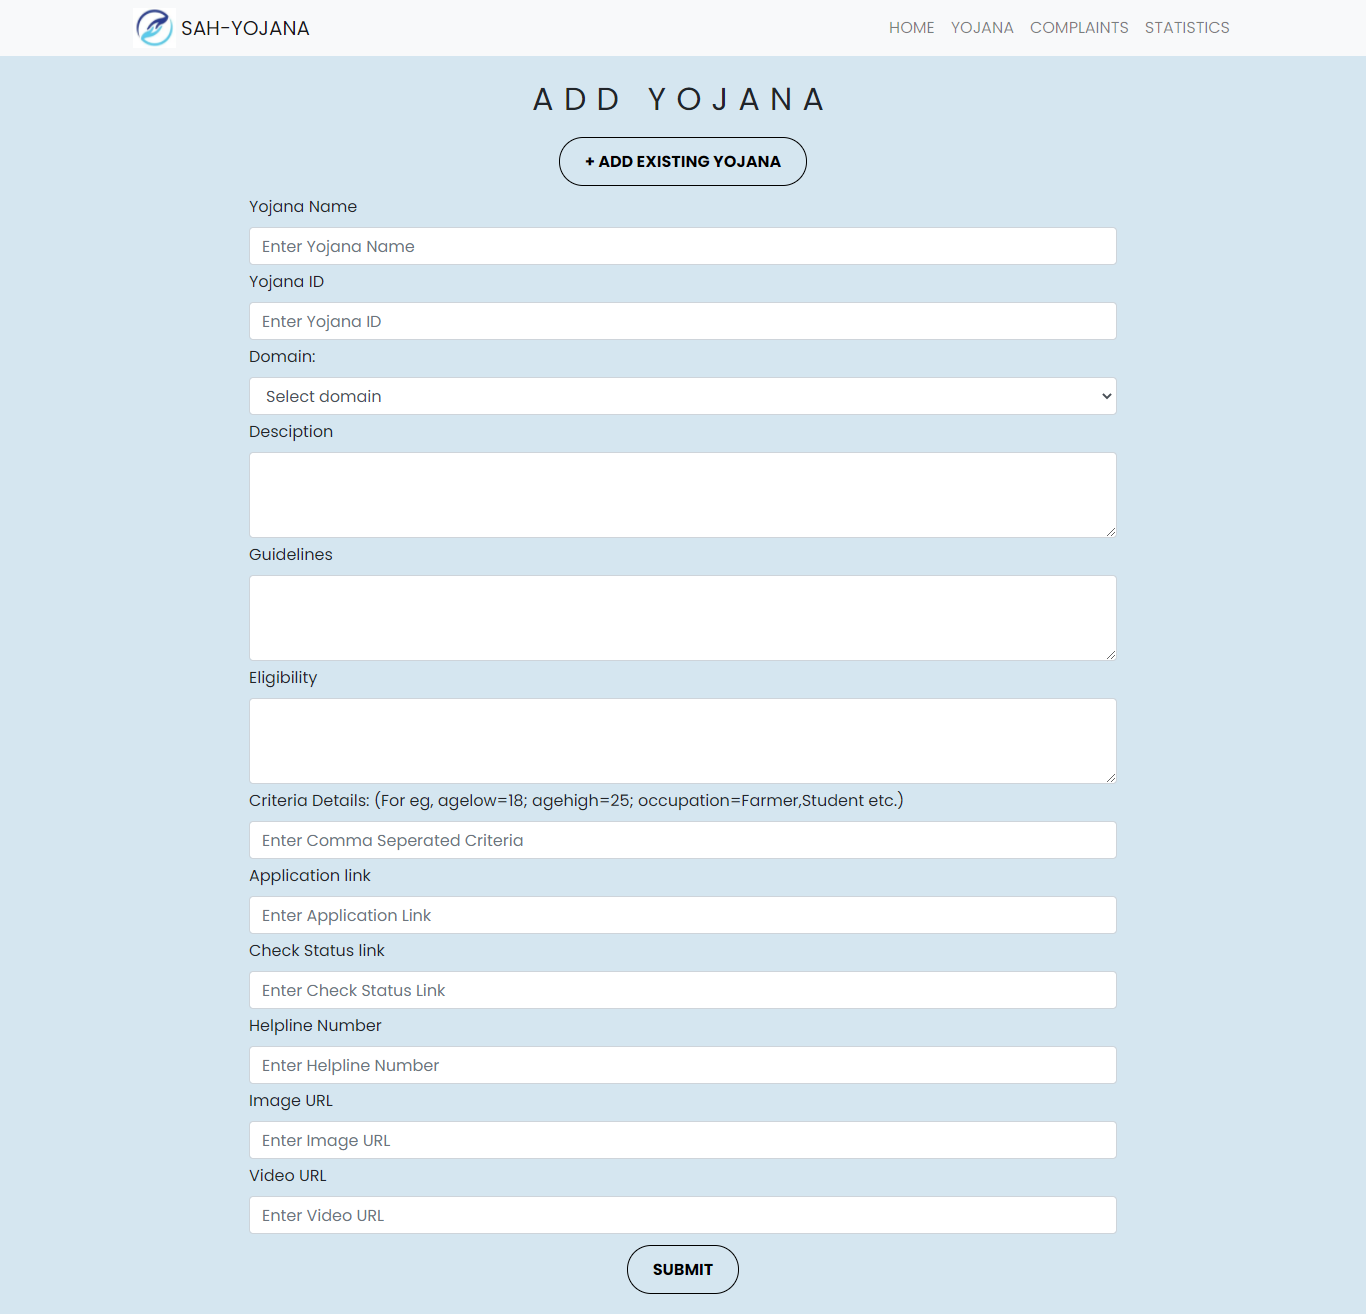
\includegraphics[width=0.45\textwidth]{add_yojana.png}}
\caption{Add Yojana page}
\end{figure}
\paragraph{Add already exisiting Yojana}
This page displays all the schemes disabled by the admin. The admin can enable any of the schemes and all the details regarding the scheme will be fetched from the database.
\begin{figure}[h!]
\centering
\fbox{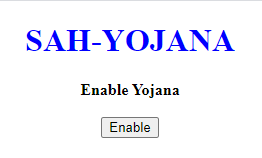
\includegraphics[width=0.4\textwidth]{Enable.png}}
\caption{Enable Yojana}
\end{figure}

\paragraph{Update / Remove Yojana}
The admin can also update an already existing scheme on the portal. The admin should click the "Update" link on the scheme card to update the details like guidelines, eligibility, description of that particular scheme. After saving the changes the user will see the updated scheme on the portal in real time.
\begin{figure}[h!]
\centering
\fbox{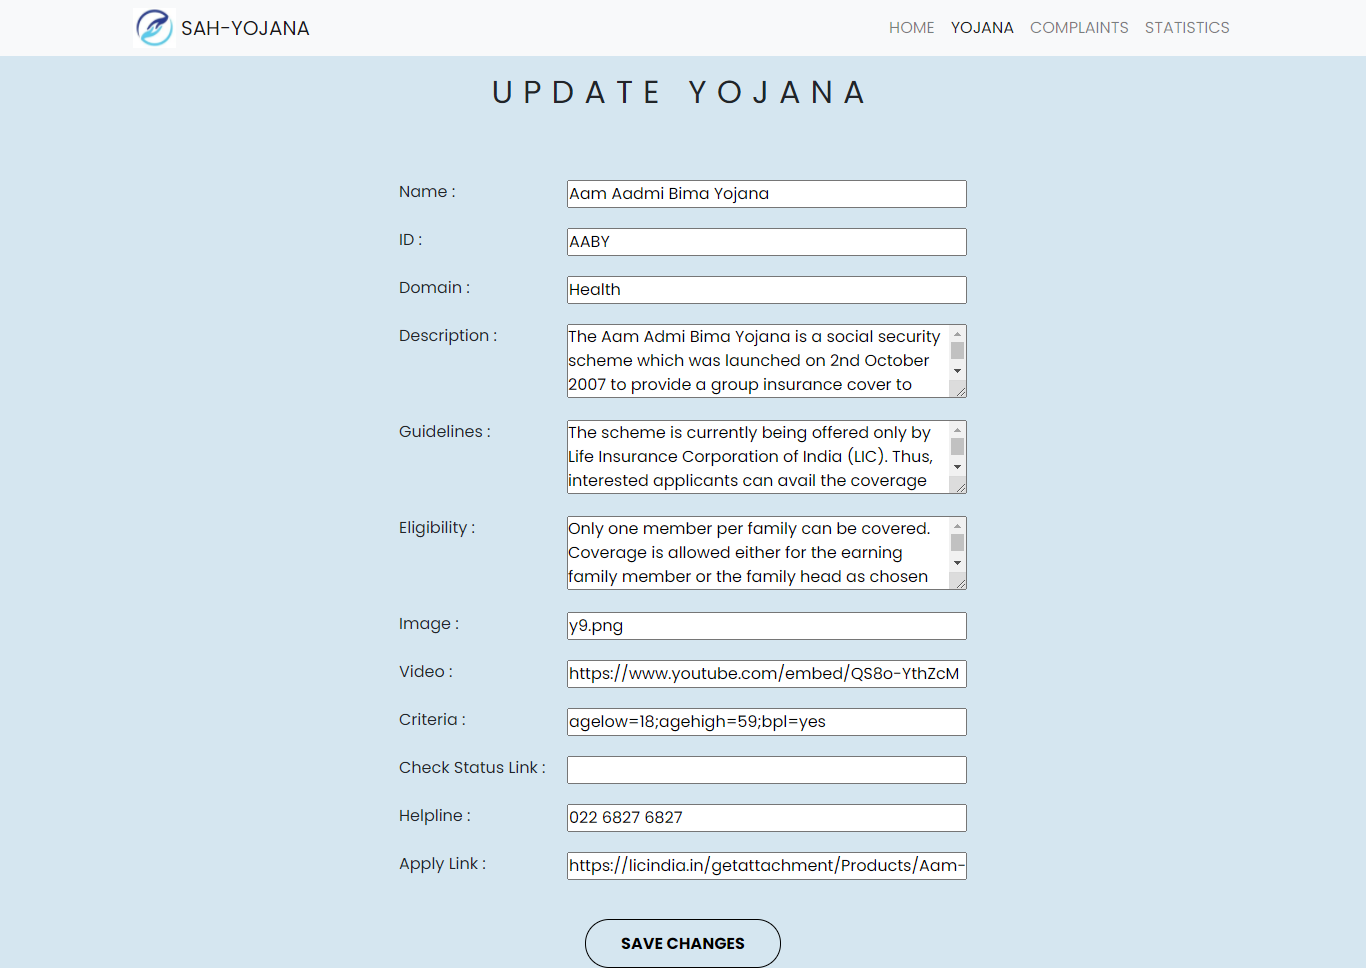
\includegraphics[width=0.45\textwidth,scale=0.45]{update_yojana.png}}
\caption{Update Yojana Page}
\end{figure}
On clicking the "Remove" link on the scheme card, the admin would be prompted with two options. The admin can either remove the scheme from the database permanently or can disable the scheme. In either case the scheme will be removed from the portal and user will no longer be able to see the scheme. The disable feature makes it easy for the admin since few schemes are activated by the government only for a certain amount of time in the year. In such cases the admin can choose to disable the scheme temporarily and enable it again when the government chooses to activate it. This saves a lot of time for the admin since the admin does not have to enter all the details of the scheme again.
\begin{figure}[h!]
\centering
\fbox{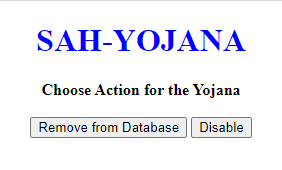
\includegraphics[width=0.4\textwidth]{Remove.png}}
\caption{Remove/Disable Yojana }
\end{figure}


\subsubsection{Statistics Page}
The admin can view various parameters and statistics related to the portal on the 'Statistics' page. It displays the following:
\begin{enumerate}
    \item Total Users: Total user registered on the portal
    \item Active Users: The number of users which are currently logged in to the portal
    \item Total Yojanas: Total number of schemes which are active on the portal
    \item Disabled Yojanas: The number of schemes which are currently inactive
    \item Total Complaints: Shows the total number of complaints lodged by the users till now on the portal
    \item Resolved Complaints: Shows the total number of complaints resolved
    \item Domain wise count of Yojanas: Shows the number of domain wise active schemes.
\begin{figure}[h!]
\centering
\fbox{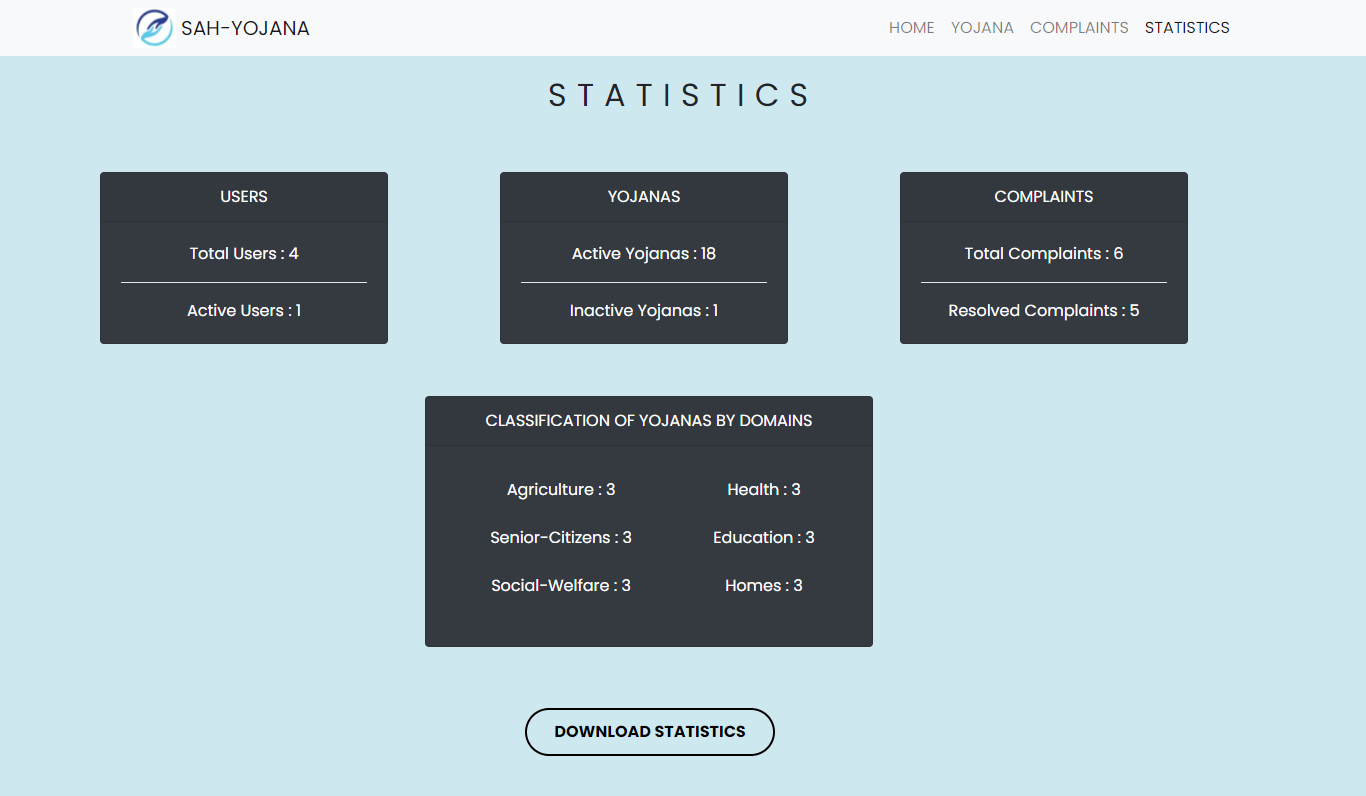
\includegraphics[width=0.45\textwidth]{statistics.png}}
\caption{Statistics Page}
\end{figure}
\end{enumerate} 
The admin can also download a report which has the count of users who have bookmarked and applied to a particular scheme by clicking on the 'Download Statistics' button. 

\begin{figure}[h!]
\centering
\fbox{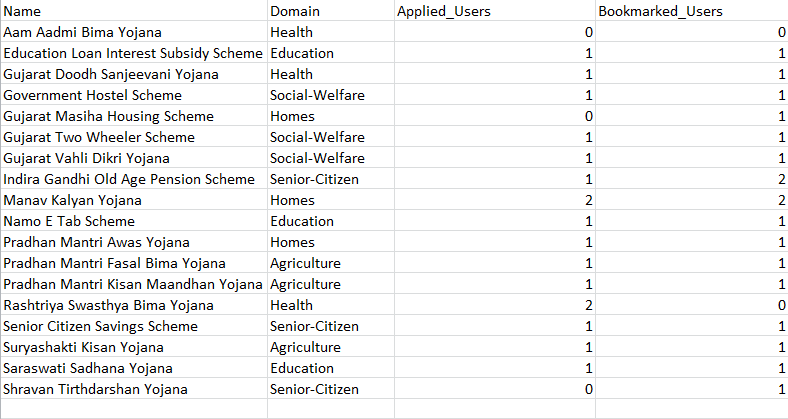
\includegraphics[width=0.45\textwidth]{snapshot.png}}
\caption{Snapshot of the downloaded excel sheet}
\end{figure}



\subsubsection{Complaint Page}
The admin can view the list of all the complaints which are lodged by the users by visiting on the "Complaints" tab in the navigation bar of the admin portal. Each complaint lodged by the user is displayed in a complain card with a brief detail about the complain. The admin can click on the card to view further details about the complain.
\begin{figure}[h!]
\centering
\fbox{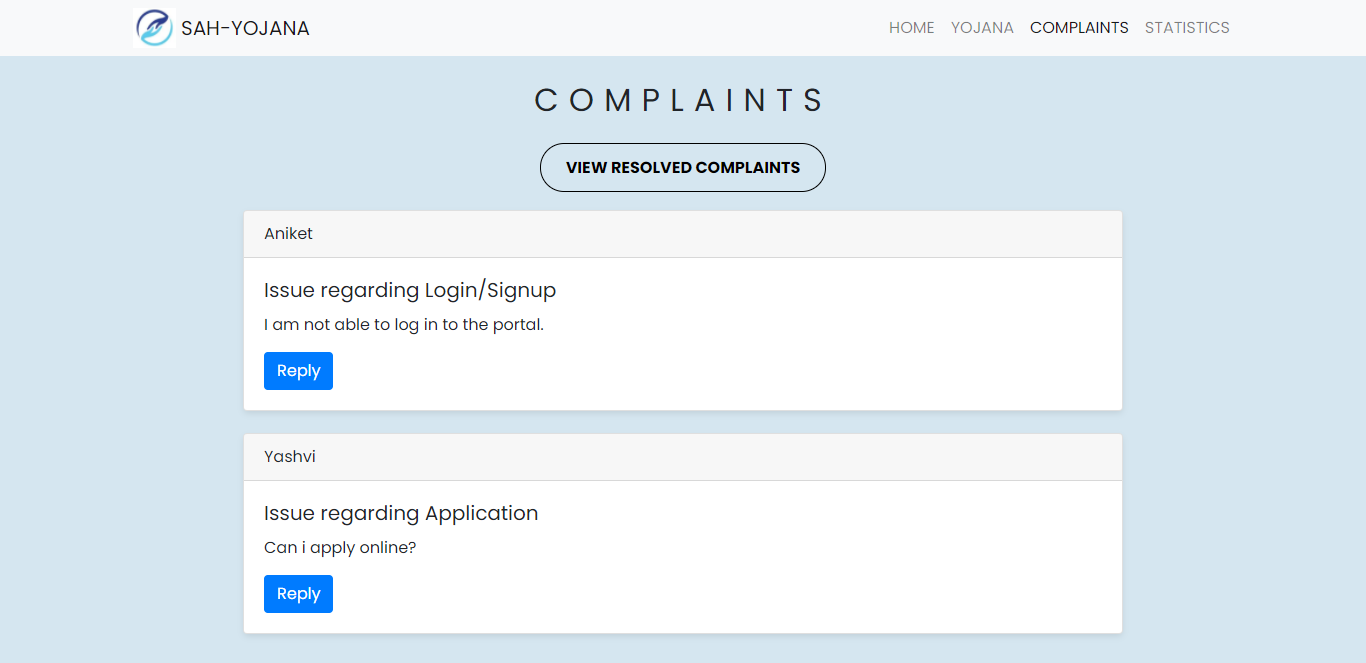
\includegraphics[width=0.45\textwidth]{admin_comp.png}}
\caption{Complaint Page}
\end{figure}
It has all the details of the complaint like the scheme name, the issue and the message mentioned by the user in the complaint. The admin can add the appropriate reply to the issue/complaint in the text box. After clicking on 'Send' button, an email is sent to the user who has lodged the complaint with the solution and the admin is prompted with "Mail sent successfully" alert. The complaint is further removed from the complaints page automatically.
\begin{figure}[h!]
\centering
\fbox{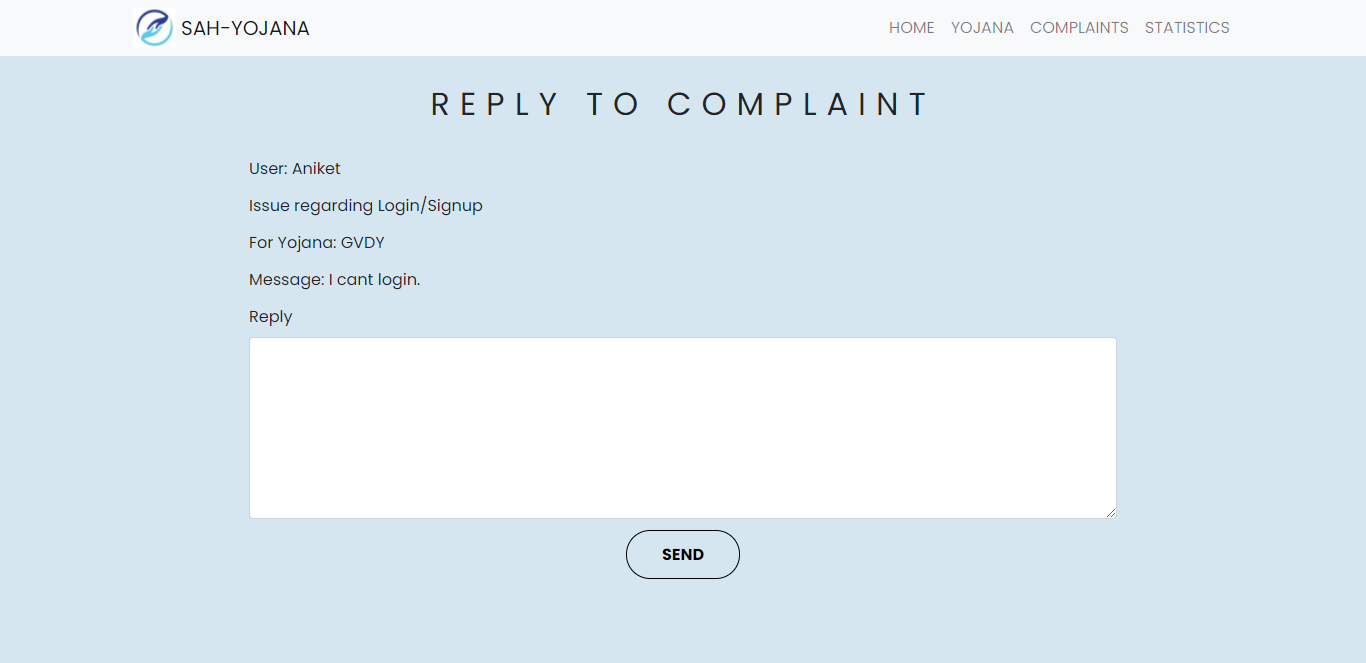
\includegraphics[width=0.45\textwidth]{reply.png}}
\caption{Reply Page}
\end{figure}
If the admin wants to view the resolved complaints then he/she can visit the "View Resolved Complaints" button which lists all the complaints that are already resolved by the user.
\begin{figure}[h!]
\centering
\fbox{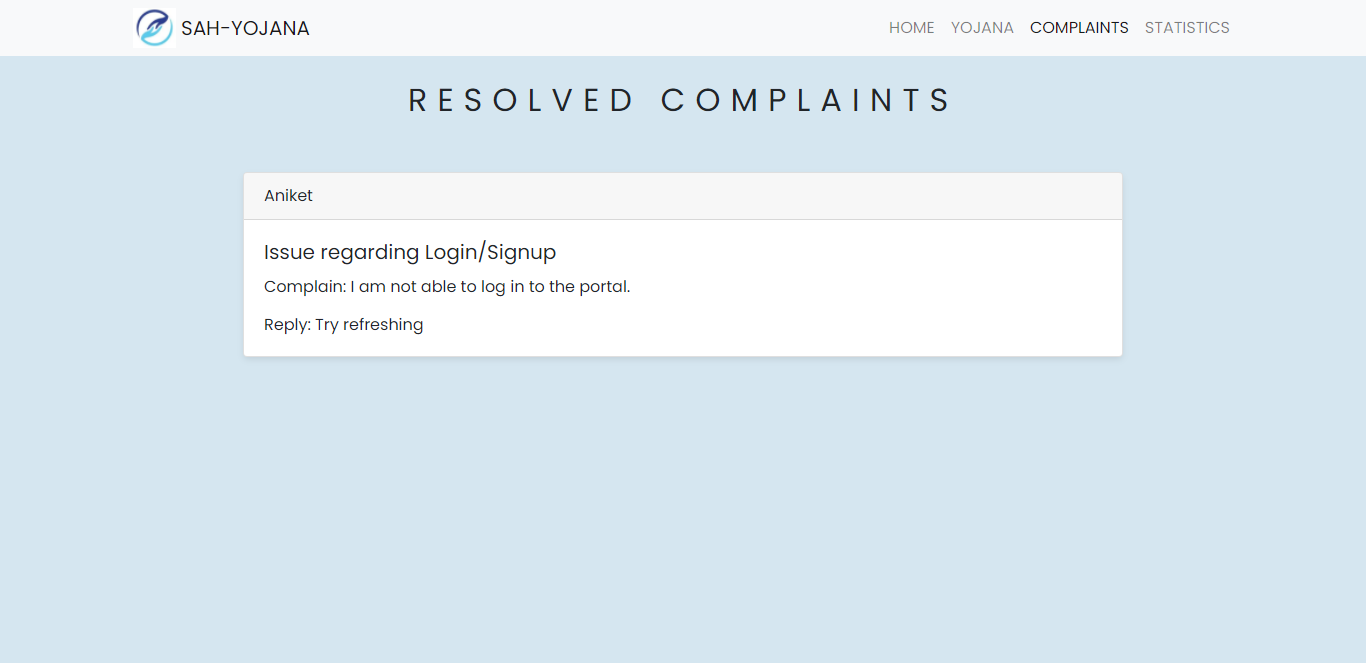
\includegraphics[width=0.45\textwidth]{resolved.png}}
\caption{Resolved Complaints Page}
\end{figure}
\section{IMPLEMENTATION}

\subsection{Design}
One of the major task in the process was to design a user-friendly and a descent UI for the website which would be easy to use for all the citizens belonging to different age groups without much trouble. A detailed plan was made describing different pages that should be a part of website and the features that should a part of the page. To get the idea of flow of the website, its UI was initially designed using Adobe XD . It is a vector based user experience design tool for web apps and mobile apps. It helps to quickly design wire frames and helps to make an interactive prototype. After that the actual implementation was started.
\subsection{Architecture}
The system follows the Model-View-Controller(MVC) framework. The view which is designed using HTML and CSS interacts and responds to the user is the major UI of the system. The controller in our system is majorly handled by Javascript which processes the logic related to the functionalities and acts as the interface between the view and the model. The model which is responsible mainly for the data flow and logic is handled by Firebase Realtime Database in our system. Fig. 25 depicts the architecture of our system.
\begin{figure}[h!]
\centering
\fbox{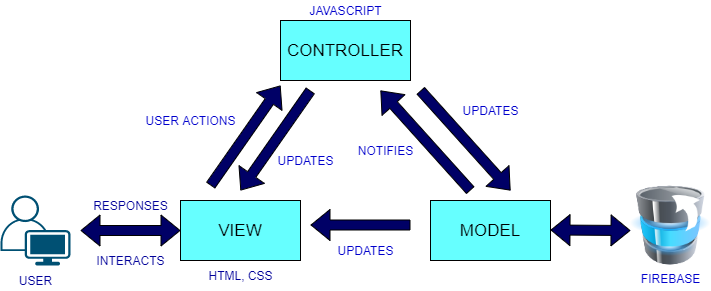
\includegraphics[width=0.45\textwidth]{MVC.png}}
\caption{MVC Architecture}
\end{figure}

\subsection{Tools and Technology}
\subsubsection{Frontend}
Front end was developed using HTML, CSS and Bootstrap. HTML was used for developing the web pages while CSS was used to control styling and layout of web pages. Further Bootstrap, a CSS framework was used to enhance the design and include responsive features like buttons and form. 
\subsubsection{Backend}
While HTML and CSS gave structure and style to web pages, Javascript\cite{b1} was used to make it interactive. Firebase Authentication was used to authenticate the users with the email ID they entered during sign up. SMTP\cite{b2} library of Javascript was used to send email notifications to the registered users. 
\subsubsection{Database}
Firebase Realtime Database\cite{b3}was used for storing the data about the users and schemes. It was used as it allows to build rich, collaborative applications by allowing secure access to the database directly from client-side code. Since complex querying was not our requirement and we needed store and sync data in real time, firebase real time database was used instead of cloud firestore. The database has three major collections namely Users, Complaints and Yojanas having their corresponding data fields. The structure of the database is as follows:
\begin{figure}[h!]
\centering
\fbox{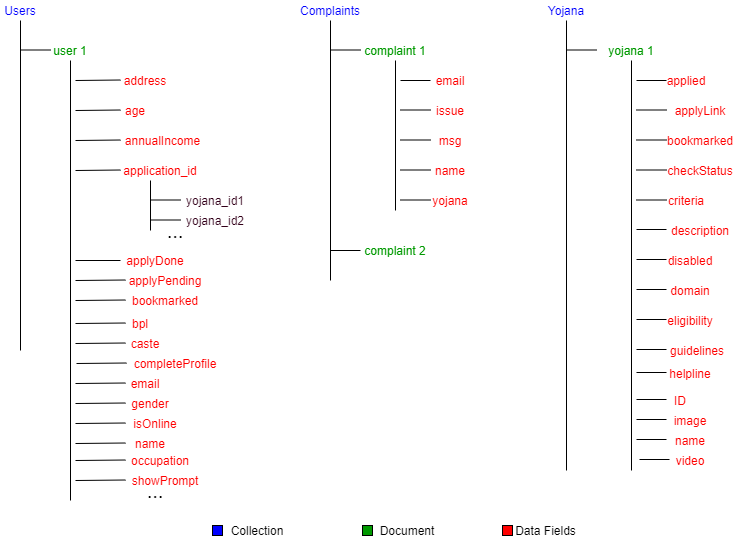
\includegraphics[width=0.45\textwidth]{Database_Design.png}}
\caption{Database Design}
\end{figure}
\subsubsection{Text Editor}
Sublime text was used for writing the code as it is a cross platform easy to use code editor.
\subsection{Testing}
After the website was developed, it was important
that the website is tested by various means.
Unit Testing is a type of software testing where individual units or components of a software are tested. We focused on unit testing right from the beginning of the development in order to eventually lead to an accurate system on its own. Once that was done, we shifted to integration testing where we tested the product directly, instead of testing the individual components and made sure that all the functionalities worked properly in the system as a whole. We took feedback from users and made changes in the portal accordingly. We went over this process over and over again and tried to make it as smooth, bug-free and efficient as possible.
\paragraph{Signup}
Table 1 lists the test cases for Sign up functionality along with the test results:
\begin{figure}[h!]
\centering
\fbox{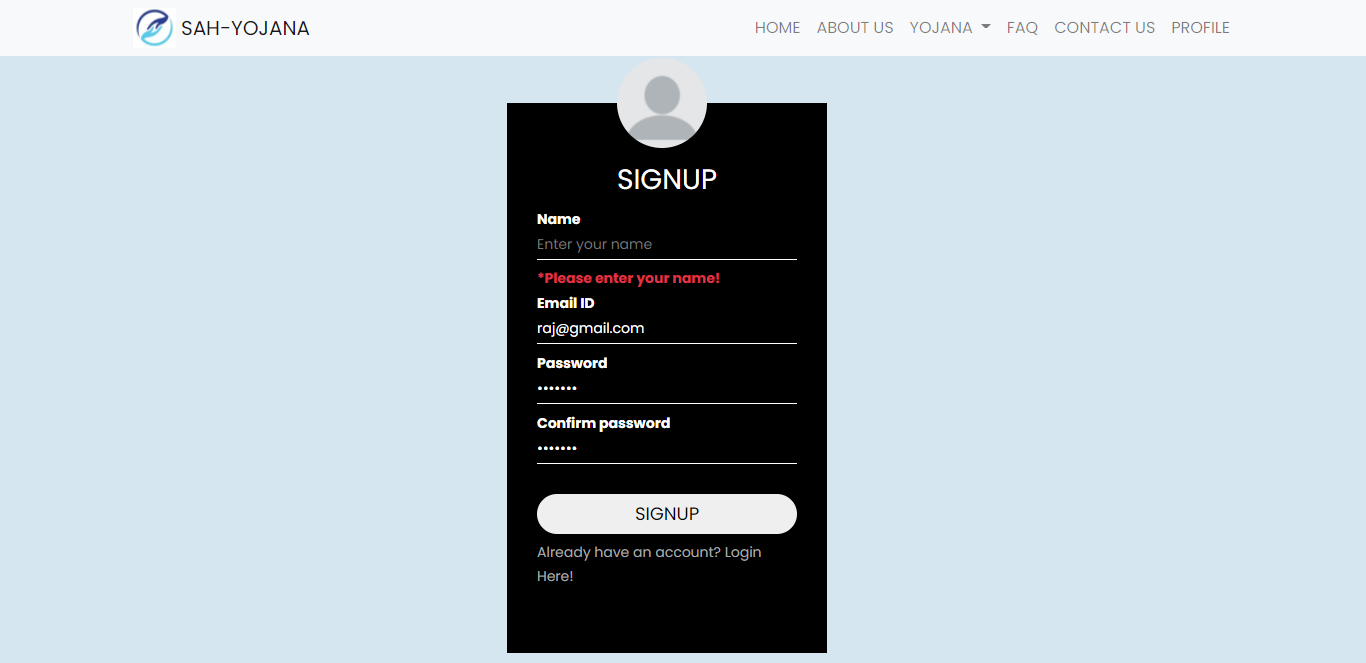
\includegraphics[width=0.45\textwidth]{empty_field.png}}
\caption{Empty field on submit for submit shows alert}
\end{figure}
\begin{table}[]
\caption{Test Cases for Signup}
\centering
\resizebox{.5\textwidth}{!}{%
\begin{tabular}{|l|l|l|l|l|l|l|l|}
\hline
\multicolumn{1}{|c|}{\multirow{2}{*}{\textbf{Action}}} & \multicolumn{4}{c|}{\textbf{Input}}                                                                                                                                         & \multicolumn{1}{c|}{\multirow{2}{*}{\textbf{\begin{tabular}[c]{@{}c@{}}Expected \\ Output\end{tabular}}}} & \multicolumn{1}{c|}{\multirow{2}{*}{\textbf{\begin{tabular}[c]{@{}c@{}}Actual \\ Output\end{tabular}}}} & \multicolumn{1}{c|}{\multirow{2}{*}{\textbf{\begin{tabular}[c]{@{}c@{}}Test \\ Result\end{tabular}}}} \\ \cline{2-5}
\multicolumn{1}{|c|}{}                                 & \multicolumn{1}{c|}{Name} & \multicolumn{1}{c|}{Email ID} & \multicolumn{1}{c|}{Password} & \multicolumn{1}{c|}{\begin{tabular}[c]{@{}c@{}}Confirm\\ Password\end{tabular}} & \multicolumn{1}{c|}{}                                                                                     & \multicolumn{1}{c|}{}                                                                                   & \multicolumn{1}{c|}{}                                                                                 \\ \hline
Wrong Email Format                                     & Raj                       & raj@com                       & rajabcd                       & rajabcd                                                                         & Please enter valid email address                                                                          & Please enter valid email address                                                                        & Pass                                                                                                  \\ \hline
Empty field on submit                                  &                           & raj@gmail.com                 & rajabcd                       & rajabcd                                                                         & Please enter your name                                                                                    & Please enter your name                                                                                  & Pass                                                                                                  \\ \hline
Password length less than 7                            & Raj                       & raj@gmail.com                 & rajabc                        & rajabc                                                                          & Password length must be atleast 7                                                                         & Password length must be atleast 7                                                                       & Pass                                                                                                  \\ \hline
Different password on submit                           & Raj                       & raj@gmail.com                 & rajabcde                      & rajabcd                                                                         & Password donot match                                                                                      & Password donot match                                                                                    & Pass                                                                                                  \\ \hline
All fields complete on submit                          & Raj                       & raj@gmail.com                 & rajabcd                       & rajabcd                                                                         & Registered successfully                                                                                   & Registered successfully                                                                                 & Passs                                                                                                 \\ \hline
Submit twice                                           & Raj                       & raj@gmail.com                 & rajabcd                       & rajabcd                                                                         & Email already registered                                                                                  & Email already registered                                                                                & Pass                                                                                                  \\ \hline
\end{tabular}%
}
\end{table}
\paragraph{Create Profile}
Testing was also performed on the profile page and following are the test cases that have been verified:
\begin{itemize}
\item Any of the field cannot be left empty on submitting else the user will be prompted to complete the field.
\item Age entered by the user should be a number only and not any alphabet.
\item Hectars of land field for the occupation farmer should also be a number and not an alphabet
\item For the fields with a drop down menu, an option from the drop down menu can only be selected.
\item On completion of the profile with all the fields completed as per the profile the data is saved successfully in the database.
\end{itemize}
\begin{figure}[h!]
\centering
\fbox{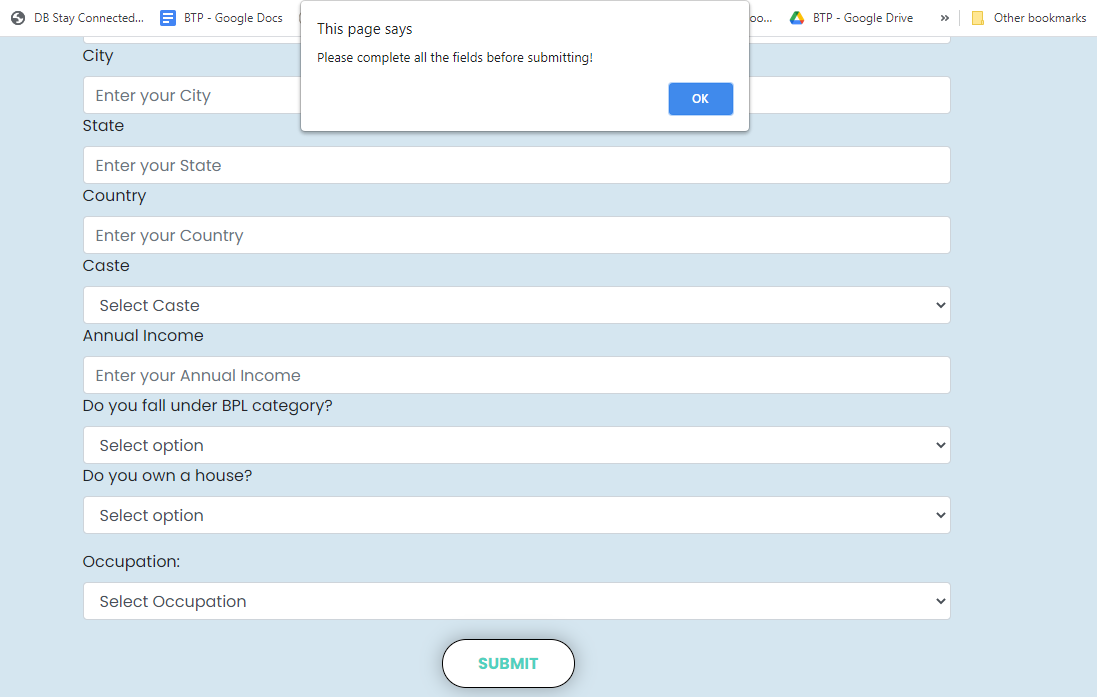
\includegraphics[width=0.45\textwidth]{profile_testing.png}}
\caption{Empty field on submit for profile shows alert}
\end{figure}
\paragraph{Recommendation}
A profile with the details as shown in Fig. 29 is created.
\begin{figure}[h!]
\centering
\fbox{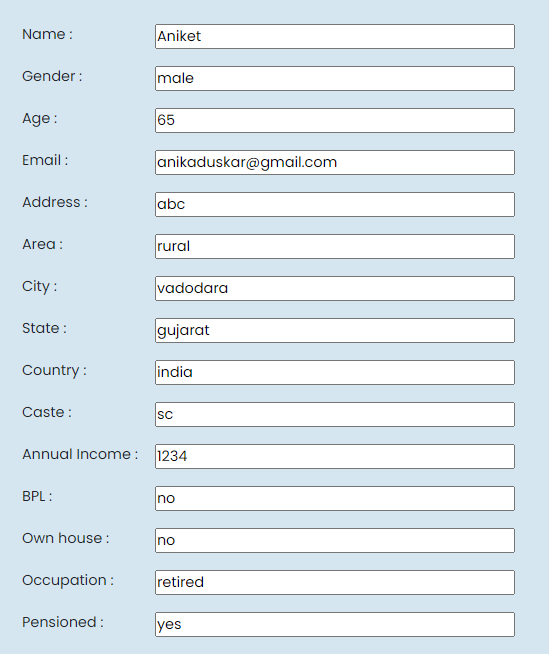
\includegraphics[width=0.45\textwidth]{Profile.PNG}}
\caption{Test User Profile}
\end{figure}
According to the profile, the following schemes should be recommended,
\begin{itemize}
    \item Shravan Tirthdarshan Yojana: The applicant should be resident of Gujarat and he/she must be atleast 60 years old.
    \item Senior Citizens Saving Scheme: A citizen having age above 55 years is eligible for the scheme.
\end{itemize}
These two schemes get recommended to the user as the profile of the user matches with the eligibility criteria of these schemes which can be seen in Fig. 30. Similarly, according to different profiles, the schemes will get recommended to the user.
\begin{figure}[h!]
\centering
\fbox{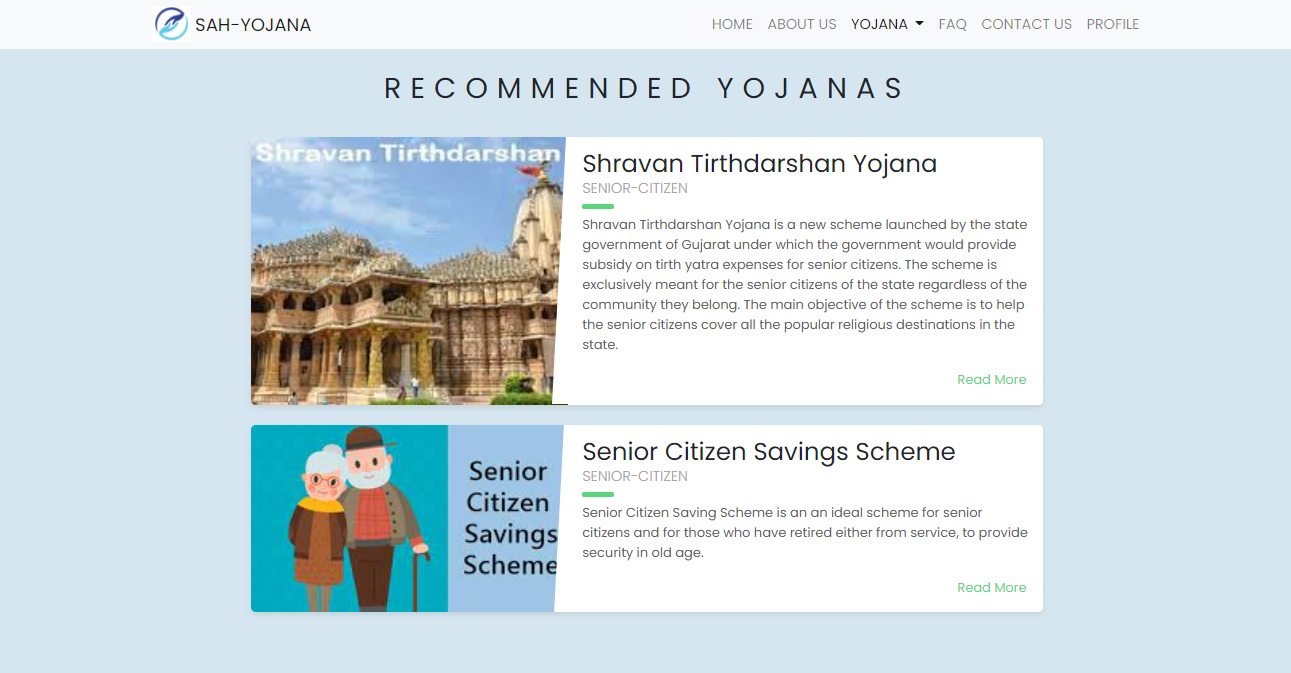
\includegraphics[width=0.45\textwidth]{recommended_testing.PNG}}
\caption{Recommended Yojanas according to the profile}
\end{figure}
\paragraph{Add complaint}
While adding a complaint, the form is validated with the following:
\begin{itemize}
    \item The email address is compulsory and should be in the correct format
    \item The issue and message should be added compulsorily
\end{itemize}
On not entering the email address in correct format, the prompt is shown as can be seen in Fig. 31.
\begin{figure}[h!]
\centering
\fbox{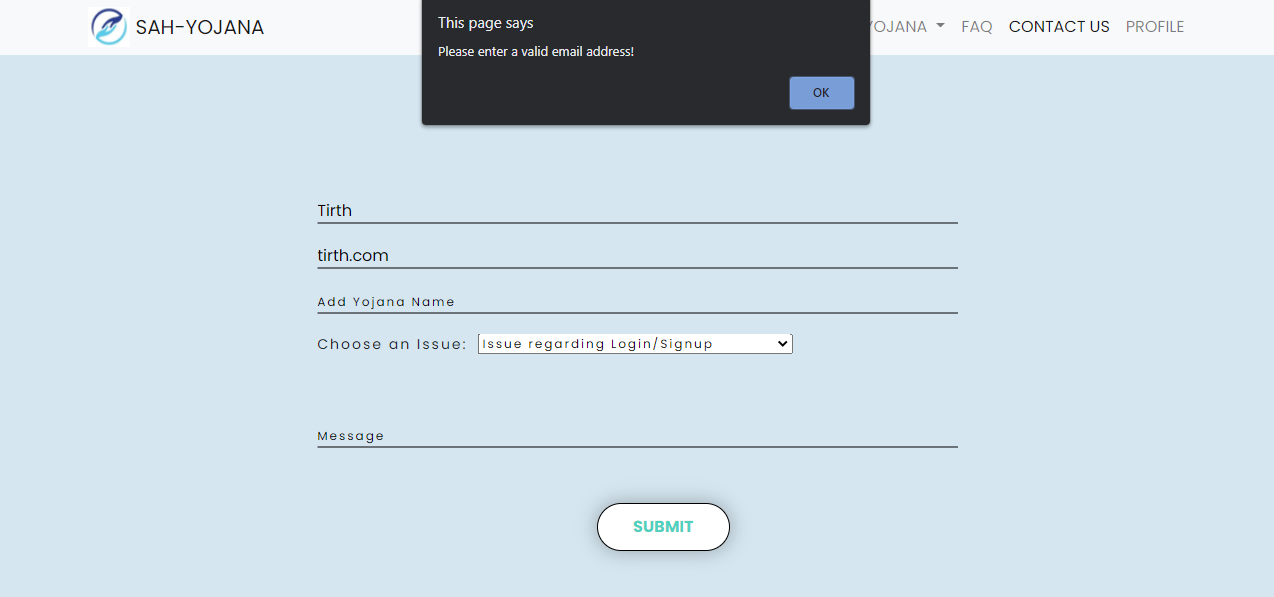
\includegraphics[width=0.45\textwidth]{complaint_testing.PNG}}
\caption{Email address not in correct format shows alert}
\end{figure}

\paragraph{Search Yojana}
When the user enters a word/letter in the search bar then all the schemes which have that word/letter in their name are shown. If no such scheme is there containing that word in its name then no scheme is displayed.
\begin{figure}[h!]
\centering
\fbox{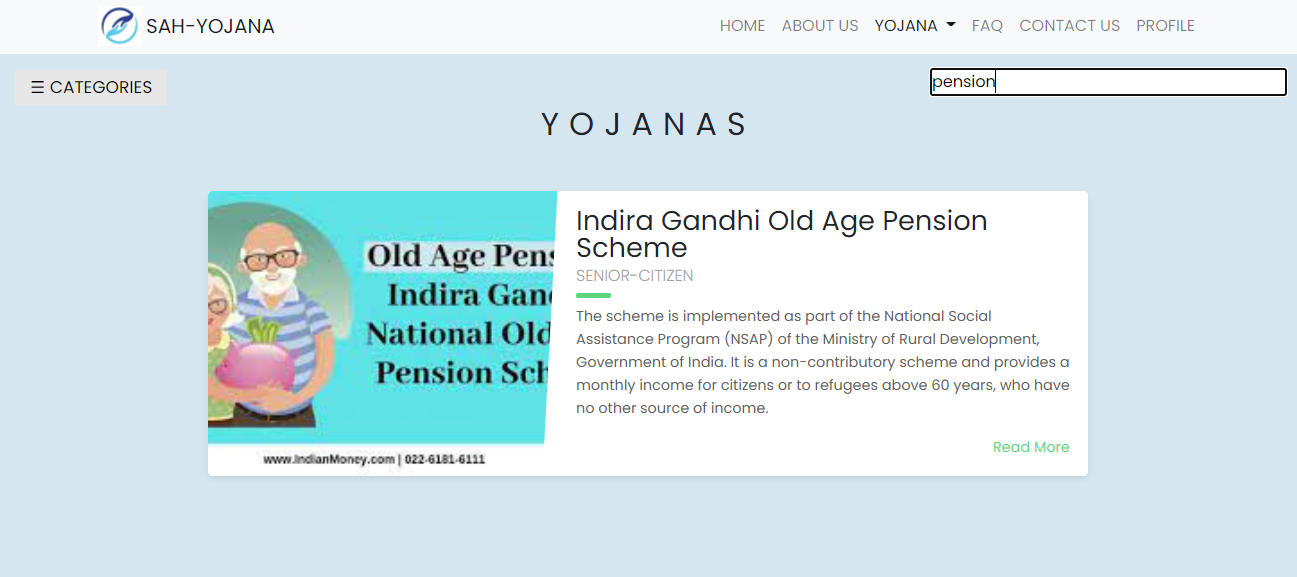
\includegraphics[width=0.45\textwidth]{search_testing.PNG}}
\caption{Yojanas having 'pension' in its name is displayed}
\end{figure}
\\The testing of other functionalities was done in the similar manner.
\section{CONCLUSION AND FUTURE WORKS}
SAH-YOJANA is a fully functional website which can recommend scheme to user according to their profile and also help them to track the application status. It helps the user for a complete process staring from the search for a suitable scheme till the benefits are received by the user. Thus the user no more has to look through 100's of website for different schemes and look through guidelines and criteria for each one of those. This saves a lot of time and also ensures that the benefits given by the government reaches its beneficiaries.
The website can be further be improved by automating the recommendation using Machine Learning Algorithms so that the recommendation can be made more accurate. 



\section*{ACKNOWLEDGEMENT}

We would like to thank Prof. Jayprakash Lalchandani for his continuous support and guidance though out the project. We would also like to thank our Prof. Gagan Garg for coordinating the complete BTP process smoothly and our university DA-IICT to provide us the opportunity of pursuing the BTP and achieving our desired targets. 


\begin{thebibliography}{00}
\bibitem{b1} Javascript Tutorial:
\url{https://www.w3schools.com/js/}
\bibitem{b2} SmtpJS:
\url{https://www.smtpjs.com}
\bibitem{b3} Firebase Documentation:
\url{https:/firebase.google.com/docs/database/}


\end{thebibliography}
\vspace{12pt}
\newpage
\section*{Appendix}
The following are the different UML Diagrams for SAH-YOJANA:
\subsection{Use Case Diagram}
\begin{figure}[h!]
\centering
\fbox{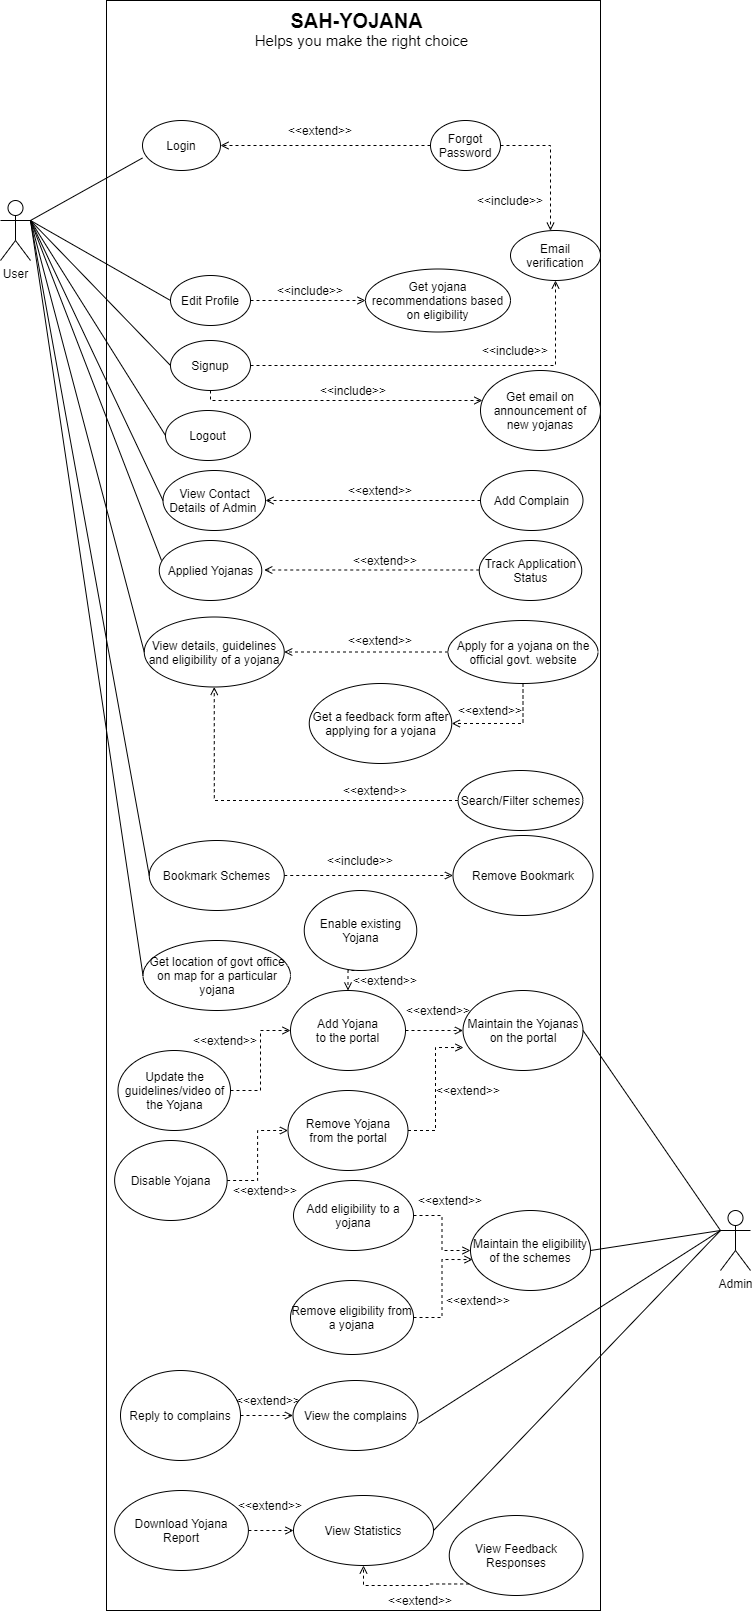
\includegraphics[width=0.45\textwidth]{Use_Case_Diagram.png}}
\caption{Use Case Diagram}
\end{figure}
\newpage
\subsection{Activity Diagram}
\begin{figure}[h!]
\centering
\fbox{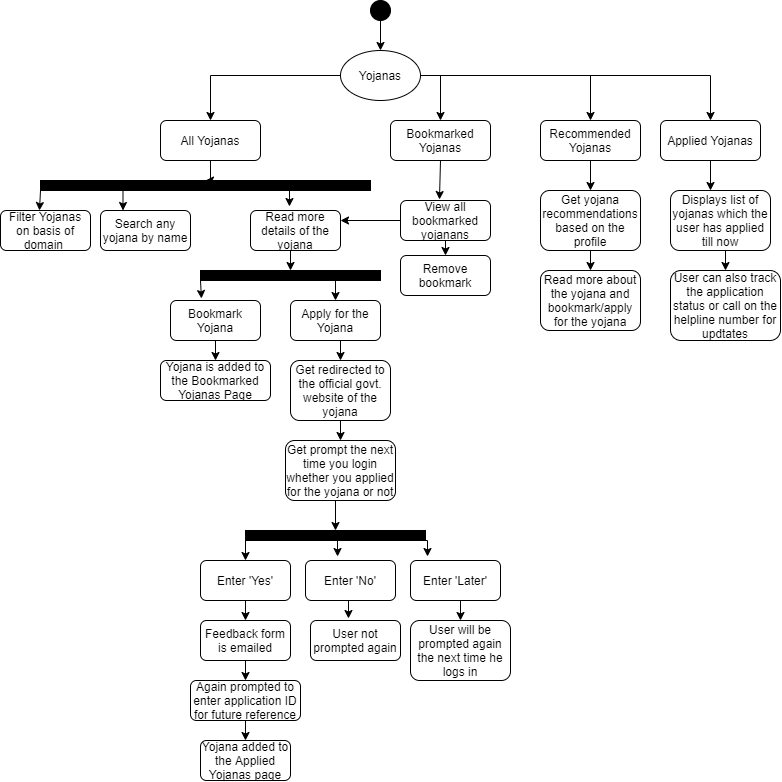
\includegraphics[width=0.45\textwidth]{Activity_Diagram_Yojanas.png}}
\caption{Activity Diagram for Admin}
\end{figure}
\begin{figure}[h!]
\centering
\fbox{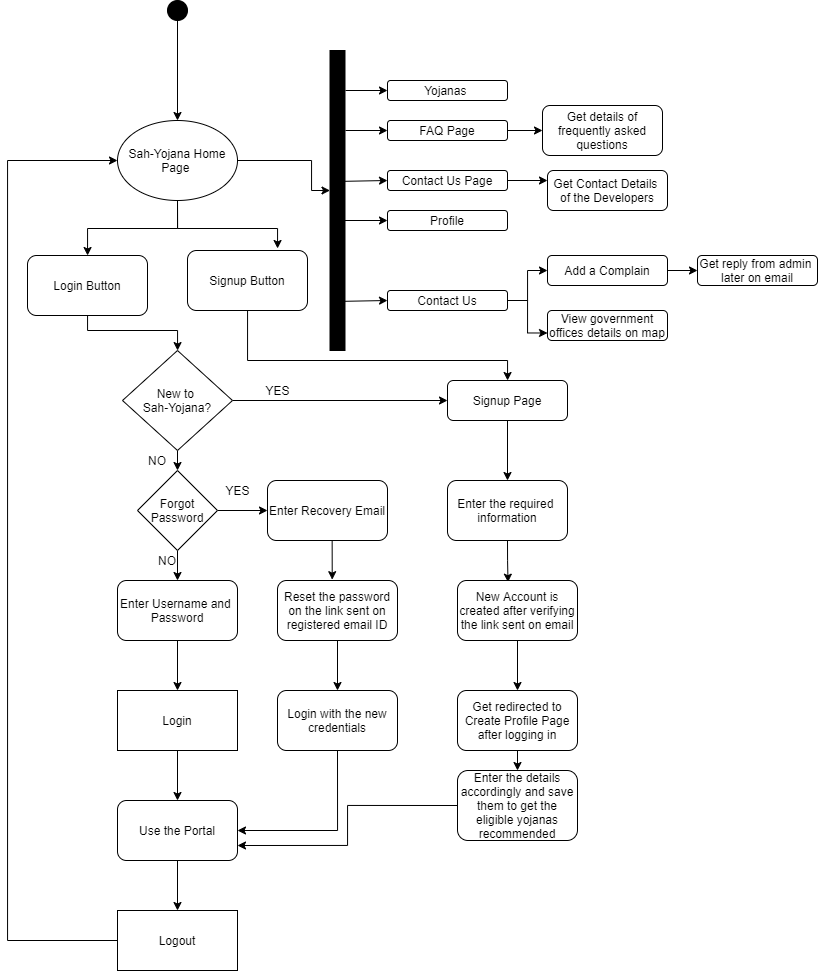
\includegraphics[width=0.45\textwidth]{Activity_Diagram_Login_Signup.png}}
\caption{Activity Diagram for Login/Signup}
\end{figure}
\begin{figure}[h!]
\centering
\fbox{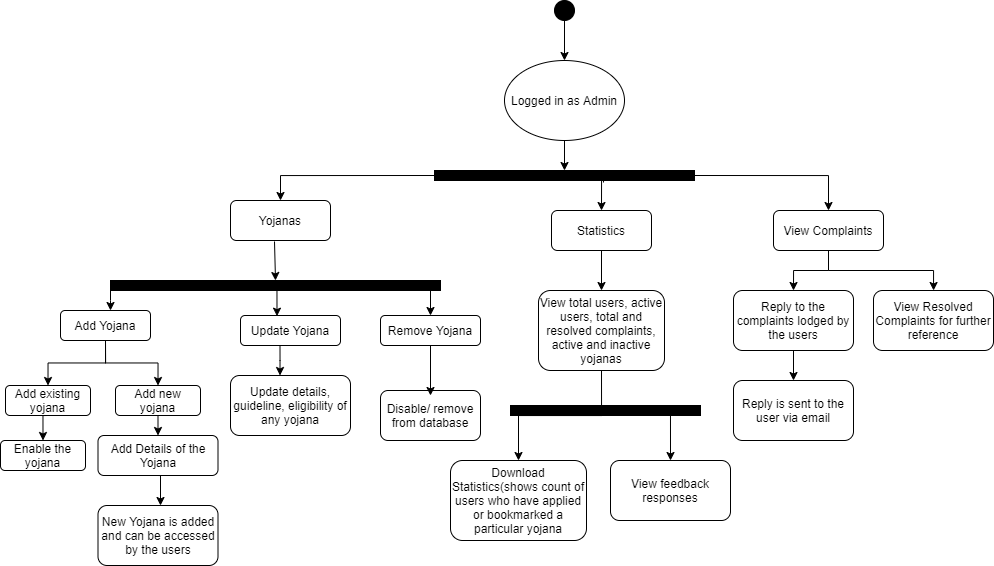
\includegraphics[width=0.45\textwidth]{Activity_Diagam_Admin.png}}
\caption{Activity Diagram for Yojana}
\end{figure}
\newpage
\subsection{Sequence Diagrams}
\begin{figure}[h!]
\centering
\fbox{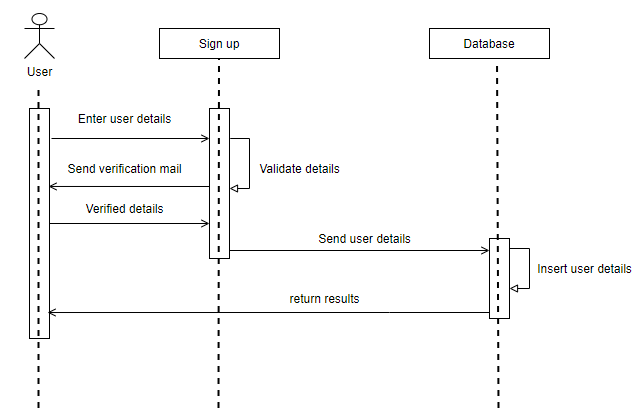
\includegraphics[width=0.45\textwidth]{sequence_signup.png}}
\caption{Sequence Diagram for Signup}
\end{figure}
\begin{figure}[h!]
\centering
\fbox{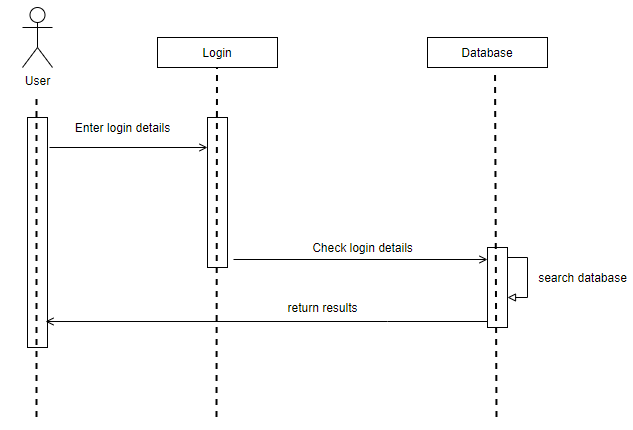
\includegraphics[width=0.45\textwidth]{sequence_login.png}}
\caption{Sequence Diagram for Login}
\end{figure}
\begin{figure}[h!]
\centering
\fbox{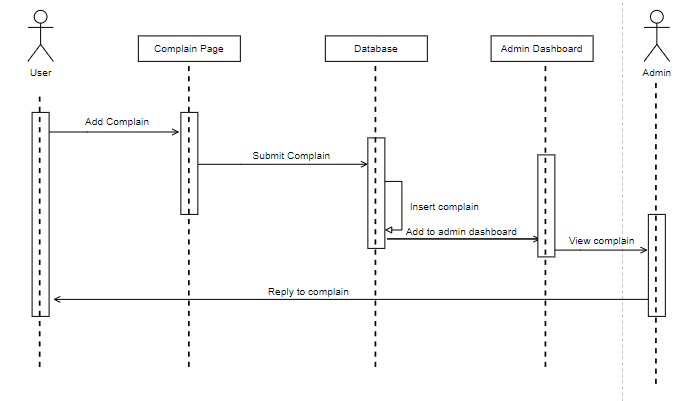
\includegraphics[width=0.45\textwidth]{sequence_complain.png}}
\caption{Sequence Diagram for Complain}
\end{figure}
\begin{figure}[h!]
\centering
\fbox{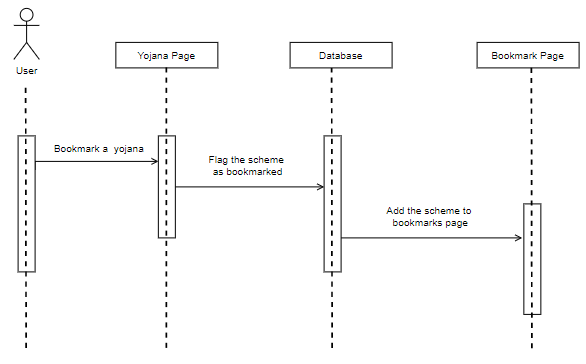
\includegraphics[width=0.45\textwidth]{sequence_bookmark.png}}
\caption{Sequence Diagram for Bookmark}
\end{figure}
\begin{figure}[h!]
\centering
\fbox{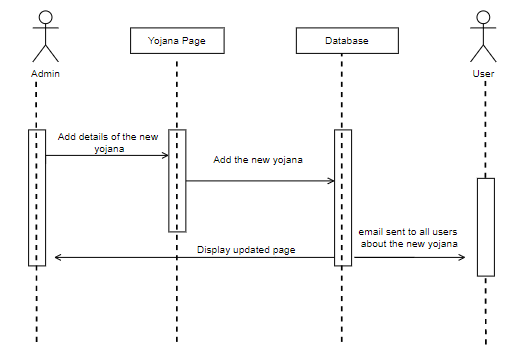
\includegraphics[width=0.45\textwidth]{sequence_newyojana.png}}
\caption{Sequence Diagram for adding a new yojana}
\end{figure}
\begin{figure}[h!]
\centering
\fbox{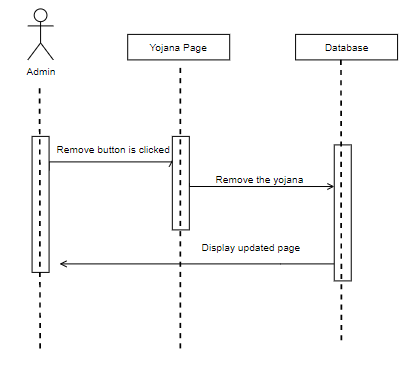
\includegraphics[width=0.45\textwidth]{sequence_remove.png}}
\caption{Sequence Diagram for removing a yojana}
\end{figure}
\begin{figure}[h!]
\centering
\fbox{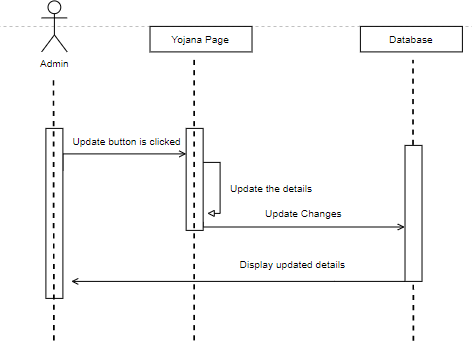
\includegraphics[width=0.45\textwidth]{sequence_update.png}}
\caption{Sequence Diagram for updating a yojana}
\end{figure}
\begin{figure}[h!]
\centering
\fbox{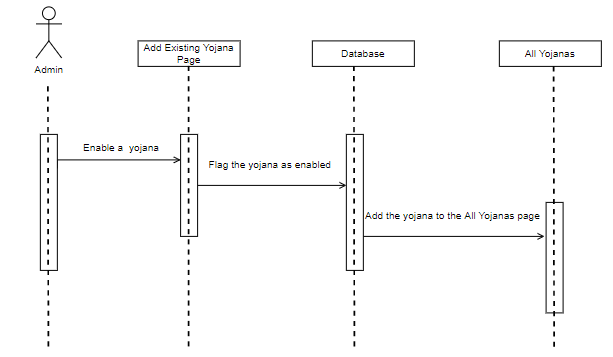
\includegraphics[width=0.45\textwidth]{sequence_enable.png}}
\caption{Sequence Diagram for enabling a yojana}
\end{figure}
\begin{figure}[h!]
\centering
\fbox{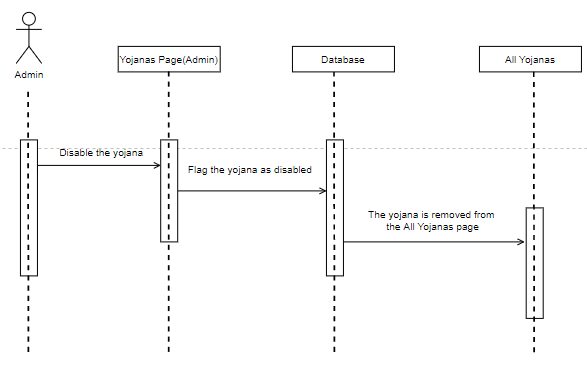
\includegraphics[width=0.45\textwidth]{sequence_disable.png}}
\caption{Sequence Diagram for disabling a yojana}
\end{figure}
\begin{figure}[h!]
\centering
\fbox{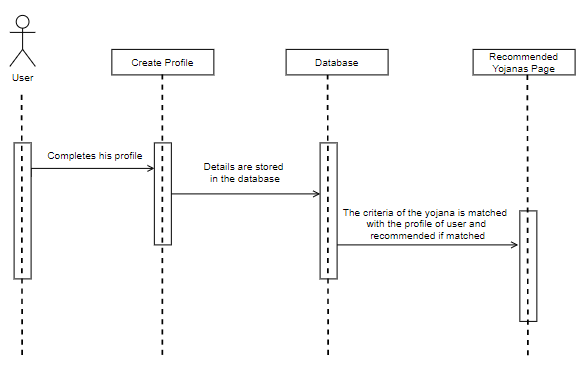
\includegraphics[width=0.45\textwidth]{sequence_recommend.png}}
\caption{Sequence Diagram for recommendation}
\end{figure}

\end{document}
